% !TEX root = ../main.tex

% = = = = = = = = = = = = = = = = = = = = = = = = = = = = = = = = = = = = = = = = = =

\section{Introductory Remarks}

Capitalization, infrastructure, and regulation make new deployments of financial technology challenging. Blockchain systems like Ethereum radically reduce the barrier-to-entry by allowing anyone to deploy any solution, provided it can operate autonomously as software. The key promise of code running on Ethereum is that the code will execute exactly as it is written, and the code that is written can never be changed. Ethereum cannot maintain this promise unconditionally but its assumptions---that certain cryptographic primitives are secure, and that well-intentioned participants outweigh malicious ones---provide a realistic level of assurance. 

The immutability of a smart contract's code is related to trust. If Alice can validate the code of a contract, she can trust her money to it and not be surprised by its behaviour. Unfortunately, disguising malicious behaviour in innocuous-looking code is possible, and many blockchain users have been victims of such contracts (`rug pulls'). On the other hand, if the smart contract is long-standing with lots of attention, and perhaps assessments from third-party professional auditors, the immutability of the code can add confidence. 

Consider the case where a security vulnerability in the code of a smart contract is discovered. The flip-side of immutability is that it prevents software updates. Less urgently, some software projects may want to roll out new features, which is also blocked by immutability. There is an intense debate about whether this is a positive or negative, with many claiming that `upgradability is a bug.' We do not take a position on this debate. We note that upgradability is happening and we seek to study what is already being done and what is possible. 

Is there a way to deploy upgradeable smart contracts if all smart contracts are (practically speaking) immutable? Consider a two simple ideas. The first is to deploy the upgraded smart contract at a new address. One main drawback to this is that all software and websites need to update their addresses. A second simple idea is to use a proxy contract (call it P) that stores the address of the `real' contract (call it A). Users consider the system to deployed at P (and might not even be aware it is proxy). When a function is called on P, it is forwarded to A. When an upgrade is deployed to a new address (call it B), the address in P is changed from A to B. This solution also has drawbacks. For example, if the proxy contract hardcodes the list of functions that might be called on A, new functions cannot be added to B. Another issues is that the data (contract state) is stored in A. For most applications, a snapshot of A's state will need to be copied to B without creating race conditions. Mitigating these issues leads to more elaborate solutions like splitting contract logic and state between different contracts, utilizing Ethereum-specific tricks (fallback functions to capture unexpected function names), and trying to reduce the inefficiencies of using a cluster of contracts.

\paragraph{Contributions.} 

\textblue{Finalize this text later.} %In the following sections we classify different ways of upgradeability on Ethereum blockchain, and describe pros and cons of each approach. Then we evaluate the upgradeability methods and compare them with each other. We conducted a measurement study in the most favorable upgrade pattern in Ethereum blockchain and give a dataset of them. Also we will talk about possible agents that is responsible for the changes on the Dapps. In the last part we will talk about some problems we are facing in the upgrade process and the ways that we can handle them.

% = = = = = = = = = = = = = = = = = = = = = = = = = = = = = = = = = = = = = = = = = =

\section{Background and Related Work}

\begin{figure}[t]
  \centering
      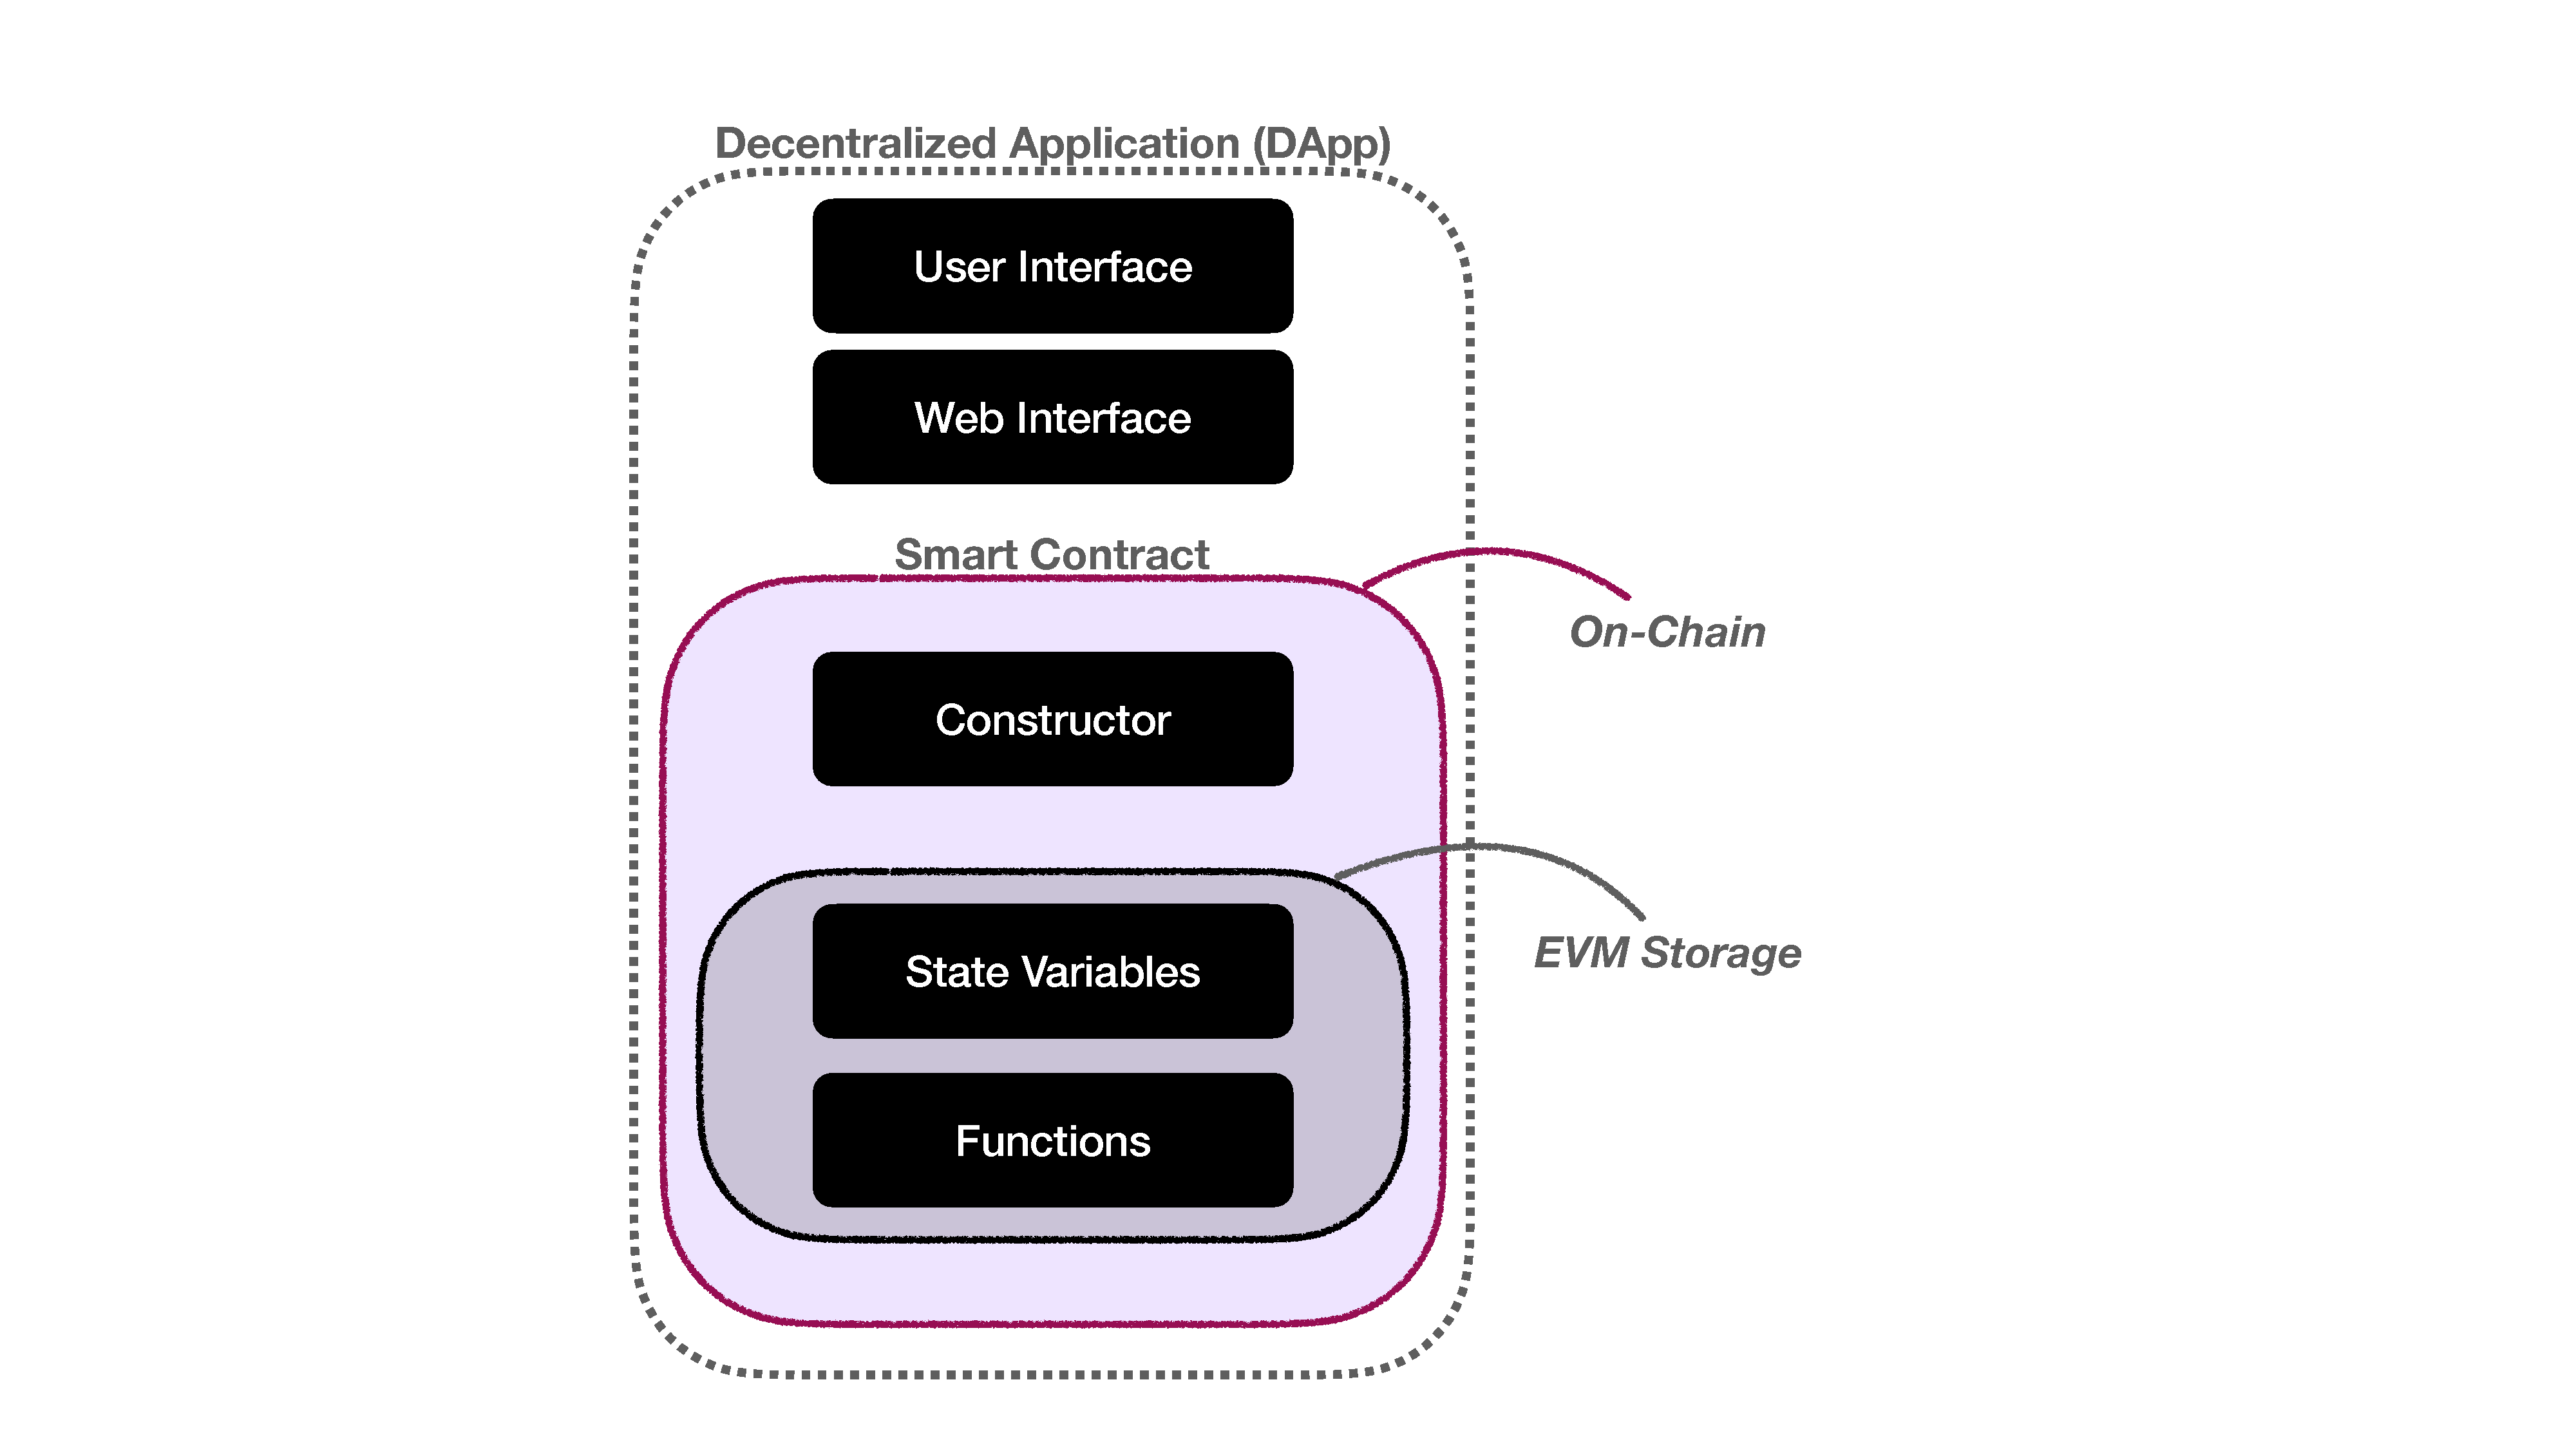
\includegraphics[width=0.3\textwidth]{figures/dapp.pdf}
  \caption{Components of a decentralized application.\label{fig:dapp}}
 \end{figure}

\paragraph{Updating vs. upgrading.} Software maintenance is part of software's lifecycle, and the process of changing the product after delivery. Often a distinction is drawn between software \textit{updates} and software \textit{upgrades}. An update modifies isolated portions of the software to fix bugs and vulnerabilities. An upgrade is generally a larger overhaul of the software with significant changes to features and capabilities. In our paper, we will only use the term upgrade and instead distinguish between retail (parameters and isolated code) and wholesale (entire application) changes. 

\paragraph{DApp vs. smart contract.} Figure~\ref{fig:dapp} shows the main components of a decentralized application (DApp). The core component is the smart contract (or simply contract), which is the set of functions and state stored on-chain. When first deployed, the smart contract also includes a constructor function which executes once and is then discarded (to be more precise, a copy of the constructor is stored in the record of transactions, called the calldata, but it is not retained in the EVM and can never be called again). While it is possible to interact directly with a smart contract by invoking its functions through Ethereum, generally users are provided an off-chain website with a user interface. Website actions are translated into calls to the Ethereum network through a set of tools (most prominently web3) in the web interface. 

While upgrades to the user interface can significantly change a user experience and expose new features, they are governed by traditional software maintenance. Our paper only considers the on-chain smart contract component, which is significantly more challenging to upgrade as it is on-chain and immutable under reasonable circumstances. 

\paragraph{Related work.} \textblue{TBD}

% = = = = = = = = = = = = = = = = = = = = = = = = = = = = = = = = = = = = = = = = = =

\section{Classification of Upgrade Patterns}

\begin{figure}[t]
  \centering
      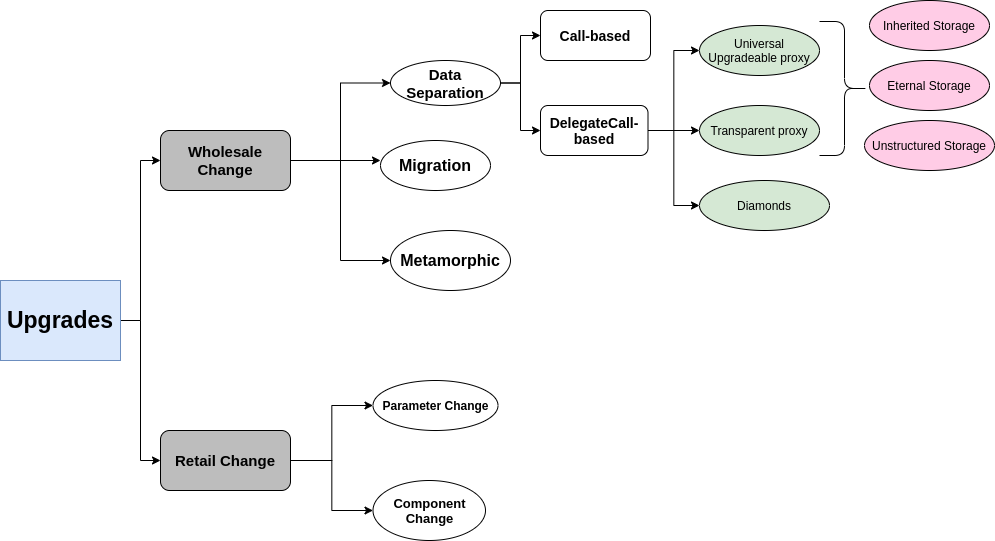
\includegraphics[width=0.8\textwidth]{figures/New_Classification.png}
  \caption{Classification. \textblue{Re-arrange to match ordering of text. Include section numbers of leaf nodes.}\label{fig:class}}
 \end{figure}
 
A variety of upgradeability patterns have been proposed for smart contracts on Ethereum. We categorize them in Figure~\ref{fig:class}. While some distinctions we make are applicable to other blockchain systems or even to software in general, the most popular approaches are leveraging Ethereum-specific operations and memory layouts.

The approaches have evolved over  time and some of them are no longer useful because of the advantages of other new methods. \textblue{Can we prove this with measurements?}

% Misc notes:
% We have some off-chain upgrades like what people did to force UNISwap using arbitrum as the L2 solution. It is an off-chain upgrade not an automated one.
% Does Factory patterns can be defined as upgradeability patterns? Like creating a new pool for Uniswap!

% = = =

\subsection{Parameter Configuration}

We first categorized upgradeability patterns into two main classes: \textit{retail changes} and \textit{wholesale changes}. A pattern for retail change does not enable the replacement of the entire contract. Rather, a component of the contract is pre-determined (before the contract is deployed on Ethereum) to allow future upgrades, and the code is adjusted to allow these changes. 

The simplest upgrade pattern is to allow a system parameter, that is stored in a state variable, to be changed. This requires a \textit{setter function} to overwrite or adjust the variable, and access control over who can invoke the function. For example, in `decentralized finance' (DeFi), many services have parameters that control fees, interest rates, liqudation levels, \etc. Adjustments to these parameters can initiate large changes in how the service is used (and its `tokenomics'). A DeFi provider can retain control over these parameters, democratize control to a set of token holders, or  lock the parameters from anyone's control. In Section~\ref{sec:governance}, we dive deeper into the question who can upgrade a contract. 

% = = =

\subsection{Tweak strategy} 

This pattern is an easy way for changing part of the code in a contract responsible for a specific feature. Instead of implementing that specific function in the main contract to take care of a specific task, the developer can deploy another contract that contains the logic needed for that part and each time the main contact needs to do the logic, it will call that specific function on the other contract and get the result of the call. By deploying a new contract and changing the pointer in the main contract, we can upgrade that specific logic of our Dapp. After upgrade the main contract will call the newly deployed contract, so we can change the logic of the function each time in a new contract.
An example for this pattern is Compound project and how they used this pattern for their interest rate model. Compound Finance is a decentralized lending platform and needs a way to calculate the interest rate for each asset on the main contract, It uses \textit{Tweak pattern} to calculate the interest rate for each asset. So if a change needed in one of the interest rate models, they can easily deploy a new contract with a new logic and then change the address which main contract uses to call and get interest rates.

% \paragraph{Pluggable Modules}. In this pattern we have a core contract that have some immutable features and then new contracts generated by the main contract and each have some or all features of the main contract. This pattern is mostly used in wallets and DeFi services like DeFi saver and InstaDapp. Users can decide to add new features into their wallet. 


%We need upgradeability to fix a bug or adding a new feature. In the event of fixing a bug, the agent who is responsible for the upgrade need to be as quick as possible to address a security issue or bug and so there is no need to have consensus of the users of the Dapp to make change. But, in the latter case the agent must get the consensus of the Dapp users to change and add a new feature, so they do not need to be quick. This fact is another paradox in the upgradeability of smart contracts because these two different events are not distinguishable before occurring and so we cannot implement two different ways of upgrading a system (one for resolving bug, and one for adding feature). So, as a system designer, if decide to add upgradeability feature should select one of these as the main goal of adding upgradeability and design the system based on that.


\subsection{Consensus Changes}

This feature is in contrast with the changing nature of software and development area. If a bug found in a smart contract there should be a way to change the code and fix the bug. In the first days of smart contract development nobody took care of this important issue which leads to loss millions of funds and even a hard fork to Ethereum blockchain known as DAO fork. These incidents show us that we need upgradeability in smart contracts more than a centralized software because if a bug happens in a smart contract we cannot restore the previous state of the software and data base because it is equal to restoring the state of the blockchain which is a very difficult (if possible). \textcolor{red}{NOTE : We can talk more about DAO hack and the race between white hackers and the attacker.there are some other similar incidents like Parity hack in the past and more recent Compound bug which was a race between people that abusing the bug and the white hackers}

This problem brought Ethereum developers to find a way to upgrade smart contracts after deployment on the main chain. This is similar to finding a way to have mutable smart contracts in an immutable blockchain which is a paradox and a group of developers are against adding upgradeability feature to the smart contracts and say the \textbf{Upgradeability is a Bug!}~\cite{Upg-Bug}.




% = = =



% JC: It seems the evaluation table will capture this. Plus are these pros/cons relative to each other or to other kinds of upgradeability (assuming the latter, it is hard to discuss until we have shown how they work). 
%The \textit{Pros and Cons} for retail changes methods are:
%\begin{itemize}
%  \item Pros
%  \begin{itemize}
%    \item Simple to implement
%    \item Easy to audit
%  \end{itemize}
%  \item Cons
%  \begin{itemize}
%    \item Cannot fix a bug
%    \item Cannot add/change Logic in Parameter Configuration
%    \item Cannot add new Logic in Tweak Strategy
%  \end{itemize}
%\end{itemize}



%TODO: Ask shayan about DeFi save and how do they upgrade their contracts.
\paragraph{Wholesale Changes}
In contrast to previous category, sometime we need to change the whole or a big part of the logic of our smart contract. This update could be a response to an incident happen to the smart contract or a planed upgrade of the system to add new features and capabilities. Before deployment, the core developer team should have a plan for the upgrade events. We categorized these types into three main classes of the wholesale changes:

% = = =

\subsection{Contract Migration}
%who will push the old data? user to provide its own data to the new version?
In the migration plan we should write a completely new contract with our desired new logic and simply deploy it to the main blockchain as a new smart contract. Some researchers suggest to call this type of upgradeability \textit{Social Upgrade}~\cite{socialUpgrade} because in most cases there is no link between different versions of a contract technically. The only way to inform users about the upgrade event is to reach out to them in social media or other platforms and aware them about the newer version of the contract.

Contract Migration is less riskier than other types of upgrades, not cost effective compare to some upgradeability types but more decentralized to the other solutions and easier to be audited. Also, it's not good for frequent updates.The other advantage of this method is that it removes transaction gas cost needed for in some patterns like proxy, registry or call-based methods.
%https://blog.trailofbits.com/2018/10/29/how-contract-migration-works/
% Migration 300,000 balances = $7500 in october 2018

In Migrating plan we need to transfer data from old contract to the new version so we should be careful to be sure that the old version have an on-chain way to read data (getter function or the variables are public). Otherwise we should manually and in off-chain manner handle the process of gathering data and pushing it into newer version. Also in the case that the we have a huge amount of data to transfer, we should send the data to the newer version in bunch of transactions that needs time. Also we need a \textit{Migrator} contract if we decided to outsource the data migration into the users.The process of storing new data in the blockchain is one of the most gas consuming actions in working with blockchains. So if we plan to do it manually, it will be expensive to transfer the data. On the other hand, if we plan to transfer data manually we should stop the old contract to be sure that the storage won't change in the process of gathering data and pushing it to the new contract. 

In migration plans, we may decide not to stop the old version. For instance in Uniswap case we have V1, V2 and V3 up and running and there is no plan to stop them. But, it may harm our system and business because our users are splitted among different versions. 

\paragraph{Data Separation patterns}

%\paragraph{Non-Solutions.} Store bytecode in a variable and execute it?

The other type of wholesale methods is to separate data and logic part of our codes so, in the upgrade event we can keep the storage contract and just deploy a new logic contract and link the storage to the new version of logic contract.
There is a debate on whether this type of upgradeability is cheaper or not in comparison to migration method. But, this method is more efficient for Dapps in which we need frequent updates. The other important issue here is who decides on the changes we need for the system which we will discuss on further sections.
Here we have 2 different choices using \textit{Call} method and \textit{Delegate Call} method to link storage and logic contracts together. We will dive deeper into these two approaches:

% = = =

\subsection{Call-based patterns}

This type is also known as data separation pattern. In this type the interaction between logic and storage contact is handled by Call opcode in Ethereum Virtual Machine (EVM). In call based patterns user is supposed to call the logic contract and the logic contract will interact with the storage by calling setter or getter function inside storage contract whenever needs to read or write a data. The logic contract is the one that should be upgraded.

The most important part in this pattern is that we cannot change the storage layout of the storage contract after deployment. So we cannot add new storage variable after the deployment. But, in most smart contracts we need to add new data for example adding the balance for new user. A solution to this problem is proposed in ERC930 or Eternal Storage pattern. Eternal storage uses mapping (key-value pair) to store data, using one mapping per data type. For instance for integer type we will define a mapping of byte32 to integer. This way we always can add new integer variables to our storage contract just by adding a variable to this mapping and having a new byte32 as key. This pattern is a good solution when we have simple data types like integer, boolean, string, etc. but it is very complex to have a eternal storage layout for complex data types such as structures, mappings or combination of them.

In this type of upgrade the address of the contract will be changed after upgrade so we need to aware our users about the change and interacting with the new version. Also it may break the compatibility of the ecosystem. In case of upgrade all smart contracts and Dapps that are interacting with the upgraded smart contract must change the address which they pointed to in order to interact with our contract. It may leads into a disaster if other contracts that are interacting with our contract do not have a way to change the address. We should also make other off-chain services (e.g. exchanges) aware of the change to start using the new version of your contract. In Call-based pattern we should have a way to stop previous version during/after upgrade because both of them are shared the same storage contract. 
There are three main ways to implement upgrades using data separation pattern. The easiest way is to change the ownership of storage contract into new upgraded logic contract and then \textit{Pause} the old contract using \textit{Circuit Breaker} pattern or set its pointer to 0x0 address. The other solution is to forward the calls receive by the old contract into the new logic contract. The last option is to set a registry contract that just keeps the address of latest version of the logic contract and call into it.


Using Calls-based pattern we eliminate the process of data migration from the old contract to the newer version and it is easy to understand this type of upgradeability pattern. But it is hard for developers to deal with this pattern when their logic contract needs complex data structures such as mapping or structures. Also the developers should change their code a lot if they decide to use this upgradeability pattern in their non-upgradeable code. 

% = = =

\paragraph{DelegateCall-based upgrades}
Similar to call based patterns here we have two contracts, Storage and Logic contract. In this pattern we may have more than one logic contract or storage contract. The difference here is that the user is calling storage contract(s) first (a.k.a proxy contract), and the proxy contract will use \textit{DelegateCall} opcode to link to the logic contract(s) (a.k.a implementation contract). In fact, there is a fallback function inside the proxy contract and inside the proxy, there is a delegate call that forwards the whole message data to the implementation contract.
The fallback functions in Ethereum will be executed if the user calls the smart contract with a function signature that does not exists on that contract.

So, if the user calls a function that does not exists on the proxy contract, the fallback will be executed and so the message data will be delegated call into the implementation contract and if the function that is called by user exists on the implementation contract the function will be executed.

So if we need to add/change the functionality of our Dapp, we just need to deploy a new implementation contract and then change the implementation address inside the proxy contract to delegate call to the new version of the implementation.

Using this pattern has two major limitations that we should take care of:

First, as described above the pattern has an assumption that the function signature of the functions inside the implementation is not existed inside the proxy contract as well. Otherwise when a user calls that function the fallback function won't be executed because the function exists on the proxy contract. So that function is not achievable inside the proxy. In Ethereum when we want to call a function we just use 4 Bytes of the hash of function name and input/output types as the function signatures. So it is possible to have 2 completely different functions with the same function signature. In the case that we have a function in implementation contract that has the same function signature with one of the functions inside the proxy we say that function signature clashes happened.

Second, the delegatecall opcode in Ethereum will run the logic of the implementation contract in the context of the proxy contract. It is similar to copy pasting the logic code into the proxy contract and altering the storage of the proxy contract. Because the delegate call opcode preserves the context, we should be sure that the storage layout of the proxy contract and the logic contract should be the same. Otherwise when we try to change a storage slot in proxy, we will end up with changing another one. The difference between storage layouts will result in a storage clashes. 


Different proxy patterns are proposed to mitigate function selector clashes and storage clashes. We will describe each of them and the advantage and disadvantages of each of them.

The first problem that we should deal with in proxy contracts is function selector clashes. In fact inside the proxy contract we need just one function called \textit{upgradeTo} function that gives the owner of the contract ability to change the address of the implementation contract inside the proxy. So in the event of the upgrade, the owner will deploy the new implementation contract and change the address variable inside the proxy to the address of the newly deployed implementation contract. By doing this the fallback function will delegate call into the newer version. So to mitigate the problem of function signature clashing we should be sure that we do not have a function with function signature equal to the functions inside the proxy, we have two main approaches to mitigate this problem:

\subsection{Universal Upgradeable Proxy Standard (UUPS)}. 
The Universal Upgradeable Proxy Standard (UUPS) method is proposed on 2019-03-04 and suggested to move the upgradeTo function to the implementation contract. So by doing this we do not have any function inside the proxy and the function signature will be mitigated. Also we reduced the size of the proxy contract. If the owner decides to upgrade the system, should call the upgrade function via calling the proxy and because the code is executed in the context of the proxy contract, the address variable of implementation inside the proxy contract will be changed.
There is a huge risk in using the UUPS proxy pattern. If the owner upgrades to a contract that does not implemented an upgradeTo functionality inside it, then the contract cannot be upgraded after that last upgrade because there is not any function inside the proxy and the latest implementation contract to upgrade the system. There is a way to check if the proposed address is a contract address and also the upgradeTo function is implemented inside that or not but that does not guarantee that the logic of the upgradeTo function is what needed to be.


\subsection{Transparent Proxy}. 
The other way to mitigate the function clashes is to check the sender of the transaction. If the owner of the contract calls the proxy the upgrade function will be executed and otherwise the fallback will be executed. This way we are sure that even if we have function clashes, then user's call will be forwarded to the implementation. 
The drawback of using Transparent proxy is that we add a check for each call to the contract which added gas cost for users on each call to the contract. (it needs to first read the address of the owner from storage which needs high amount of gas and then a check that if the sender is owner or not). 


There are three different methods to mitigate the risk of storage clashes.  To mitigate storage clashes we have three different approaches :

\subsection{Inherited Storage}. 
In this method the proxy and all logic contracts are inherited from a storage contract that contains storage variables. If we decided to upgrade the contract, we should be sure that the new implementation contract is inherited from the storage contract. Using this method we are confident that the proxy and logic contracts are using the same storage layout and storage clashes will be mitigated.
Also if after deployment we need to add new storage variables, we should just deploy a new storage contract that inherited from the previous storage contract and add the new variables to it. We should be sure that the future implementation contracts will inherit the latest storage contract. This adds-on to the inherited storage contract is called append-only pattern.
This method is not efficient because of variables that declared but not used in some logic contracts. On the other hand, each logic contract is coupled with a storage contract and it is hard to take care of this track. Also we should take care of upgrading the system each time to be sure that the new implementation contract is inherited from the latest version of storage contract.

\subsection{Eternal Storage}. 
As described before in Eternal storage, we defined mappings for all variable types that we need to use in our logic smart contract. For storing mapping variables EVM selects random slots on the storage based on the variable's name so we can mitigate the clashes using this randomness.
The main problem of this type is that the logic contract and all other contracts that are using the storage must use the mapping structure to access the storage variables and use complex syntax whenever they want to access a variable. This also results in the gas usage inefficiency because we need to call and update a mapping each time we need to change a variable.  


\subsection{Unstructured Storage}. 
The other way of mitigating the storage clashes is to assign some randomly selected slots to critical variables like address of logic contract. For instance, openzeppelin uses hash of "org.zeppelinos.proxy.implementation" to store the address of the logic contract in this slot.
The downside of this approach is that we need getter and setter function for each variable. We also can use unstructured storage for simple variables and not for mapping and structures. EIP-1967 proposed to assign specific storage slots for address variable inside the proxy contract to store the address of the implementation contract inside the proxy. The proposed slot is 0x360894a13ba1a3210667c828492db98dca3e2076cc3735a920a3ca505d382bbc which is calculated from this equation
bytes32(uint256(keccak256(eip1967.proxy.implementation)) - 1)). 
%% Add exact gas cost from the image

There are two other upgradeable proxy patterns that are proposed to address problems in some specific applications. We will describe them bellow: 

\subsection{Beacon Proxy}. 
In some type of applications such as wallets, the logics needs to make the data of each user separate. There are some proposals such as EIP-1167 or minimal proxy suggested creating a proxy contract for each user that delegate calls to the main implementation contract. Using this approach each user has its own data inside its proxy contract. The problem of using the minimal proxies is that they are not upgradeable. If a bug found in the implementation contract then all proxy instances are prone to the attack. The problem of using the previous types of the upgradeability patterns is that unlike the previous ones that have just one proxy contract and easy to change the address variable inside them, here we have tons of instances and we cannot change all address variables inside all proxies. 

Beacon proxy method is suggested to solve this issue. In beacon proxy, each proxy instance will call a registry-like contract and ask it for the latest version of the implementation contract and then will delegatecall to the resolved address. In the upgrade event, the owner needs to just change the address inside the beacon contract so all proxy instances will use the newer version of implementation contract each time calling the beacon contract and asking for the implementation contract address.

\subsection{Diamonds}
The EIP-2535 or Diamonds proxy is proposed on 2020-02-22 and suggested using multi implementation contracts with a single proxy contract. In the proxy there is a access control structure in which there is a mapping between each implementation contract's address and the function signatures that are implemented inside that specific implementation contract. Using this method we can have a separate implementation contract for each functionality of the Dapp. It will help to make the contracts more modularize. Also we can just update one functionality in each upgrade event. It also helps with the situation that the contract code size exceeds the limitation (24KB) by splitting it into a number of implementation contracts.

The drawback of using Diamonds is adding more complexity to the system because using different implementation contracts will increase the chance of storage clashes and error in handling the shared storage between them.

% = = =

\subsection{Metamorphic Upgrades (Create2-based approach)}
This type of upgradeability is relevant to \textit{Create2} opcode which is proposed by Vitalik Buterin in 2018-04-20 as EIP-1014. To create a new contract in Ethereum blockchain we have 2 different opcodes; Create and Create2. The main difference between these two is the address of the contract that is going to be deployed. In Create opcode the address depends on the address and nonce of the creator. Nonce is a number regarding to the account and is like a counter to the number of transactions sent by that account (for contract account nonce is the number of contracts that are deployed by that contract). The problem of using Create opcode for contract deployment is that we cannot have a way to calculate the address of deployed contract because it depends on the nonce of the sender. Create2 opcode solve this problem because the address of the deployed contract just depends on the address of deployer and the \textit{Bytecode} of the contract to be deployed (and also a salt number which the deployer should specify each time). So we can hardcode the address of the deployed contract before deployment if we uses Create2.

The other important property of Create2 opcode is that it uses \textit{init code} as the bytecode to calculate the address for deployment. The init bytecode is the bytecode which the creator will send to Ethereum blockchain and it is different from the \textit{Runtime Bytecode}. In fact, the EVM will execute constructor before deployment of the contract and then change the bytecode to the runtime code so the main difference between init bytecode and runtime bytecode is the constructor.

In Metamorphic upgrade pattern, we abuse the Create2 opcode and take advantage of the difference between init bytecode and runtime bytecode to redeploy a contract with a new logic in the same address. To describe the process completely we should describe the Metamorphic Contract Factory a bit. This factory contract clones the implementation contract in its constructor and deploy the new bytecode on the previous address. The key idea is that the bytecode that we are going to deploy has a constructor that changes the bytecode to what we want to be deployed. So the init bytecode is the same as the previous deployment but the runtime bytecode is the new bytecode that we want to deploy.

There is a critical point here. Before deploying a new contract on that exact address, the previous contract should be self destructed. Note that self destruct will wipe out the storage of the contract. So, in metamorphic upgradeability pattern we will lose the data and so we should migrate the data manually after deployment. In fact this type of upgradeability pattern is good for stateless contracts or contracts that has a limited storage variables (e.g. Beacon contract). The greatest risk to this type of upgradeability pattern is that there is a huge debate on the Ethereum community to remove the self-destruct opcode and without the self-destruct opcode the pattern is broken. 

In comparison to the proxy patterns, metamorphic pattern is more gas efficient because we don't need to have any checks like what we had in transparent proxy or also we don't have the delegate call process. Similar to proxy contract, after upgrade the address of new version is not changed but we need to migrate the old data to the newer version. Also in metamorphic pattern there is downtime to the system because we should firs self-destruct the previous contract and the process of self-destructing occurs at the end of the transaction. So, we should first self-destruct the old version in a transaction and then redeploy the contract in another transaction and there is a downtime between these 2 transactions.

%% add this as citation to the fact that selfdestruct will be removed: https://www.reddit.com/r/ethereum/comments/lx32kv/expectations_for_backwardsincompatible_changes/







 %%%%%%%%%%%%%%%%%%%%%%%%%%%%%%%%%%%%%%%%%%%%%%%%%%%%%%%%%%%%%%%%%%%%%%%%%%%%%%%%%%%%%%%%%%%%%%%%%%%%%%%%%%%%%%%%%%%%%%%%%%%%%%%%%%%%%%
 %%%%%%%%%%%%%%%%%%%%%%%%%%%%%%%%%%%%%%%%%%%%%%%%%%%%%%%%%%%%%%%%%%%%%%%%%%%%%%%%%%%%%%%%%%%%%%%%%%%%%%%%%%%%%%%%%%%%%%%%%%%%%%%%%%%%%%


 \section{Evaluation of different methods}
 In this section we compare and evaluate different methods discussed in previous section and explain the consequences regarding each method to the users and developers of Dapps.
 \subsection{Criteria}
 There are some characteristics that can help the designer to decide which method should be used on the system and add upgradeability to the Dapp. In this part we pencil out these criteria and evaluate different methods based on these criteria. In this part we describe and specify what it means that each row of our table receives a check mark (\checkmark), double check marks (\checkmark\checkmark), square (\XBox) or nothing. 
 
\subsubsection{Can replace entire logic}
An upgradeability method in which the upgrader is able to replace the entire logic of the system earns a check mark(\checkmark) otherwise it receives nothing.

\subsubsection{can replace pre-specified part of logic}
An upgradeability method in which the upgrader can change \emph{just} pre-specified part of logic of the system (and not entire logic) earns a check mark(\checkmark) otherwise it receives nothing.

\subsubsection{Replace entire state}
An upgradeability method in which the upgrader can replace the entire state in newer version earns a check mark(\checkmark) otherwise it receives nothing.

\subsubsection{can change pre-specified state variables}
An upgradeability method in which the upgrader can \emph{just} change some pre-specified state variables receives a check mark (\checkmark) otherwise it awarded nothing.

\subsubsection{No need to deploy a new contract}
In some upgradeability patterns, the upgrader needs to deploy a new smart contract in the process of upgrade which receives nothing. Upgradeability methods which do not need to deploy a new contract for the process of upgrade receive a check mark (\checkmark).

\subsubsection{No need to migrate state from old contract}
In some patterns, there is no need to collect data from the old version and push it to the new contract which receive a check mark (\checkmark). On the other hand, patterns which required to migrate data from old version receive nothing.

\subsubsection{No need to separate State and Logic}
An upgradeability pattern that does not requires separation of logic and storage contracts awarded a check mark (\checkmark) otherwise it receives nothing.


\subsubsection{DelegateCall opcode Risks}
Some of the upgradeability methods utilize \textit{Delegate call} opcode. Using  this opcode bring complexity to the system and needs more security considerations. These security considerations are categorized into two main risks which we explained before; function selector clashes and storage clashes.

\paragraph{Function Selector Clashes Risk}
Upgradeability methods in which the developer should take care of function selector risks receive check mark (\checkmark), otherwise receive nothing. 

\paragraph{Storage Clashes Risk}
Upgradeability methods in which the developer should take care of storage clashes risks in two contracts receive check mark (\checkmark), and the methods that the developers must consider this risk and deal with it in more than two contracts receive double check marks (\checkmark\checkmark) otherwise receive nothing. 

 \subsubsection{No indirection}  
 Indirection happens if the first external message need be forwarded from a contract to another. Upgradeability methods that do not need any indirections receive a check mark (\checkmark). An upgradeability pattern that contains indirections which adds an extra gas because of adding one or more layers of indirection awarded nothing. An upgradeability method in which just a portion of its transactions (and not all transactions to the contract) need indirection receive square (\XBox). 

\subsubsection{User endpoint address not changed}
In some upgradeability methods, after the upgrade process, users must call a new contract address to use the Dapp. It is equivalent to having 2 different Dapps at the  end of the upgrade. Alice uses a DApp X which uses one of the upgradeability patterns at address A before the upgrade. After upgrade, she may be unaware that upgrade happened and use the previous address (receive check mark (\checkmark)) or she may need to use address B instead which receive nothing.


\subsubsection{Downtime in upgrade events}
Patterns which we will have a downtime of the Dapp in the upgrade event receive check mark (\checkmark) otherwise it receives nothing. 


\subsubsection{No need to change code to add the upgrade pattern}
Upgradeability patterns in which the developers do not need to change any part of the original code to add the upgrade method receives nothing. The methods in which the developers do not need to change the whole code but should add a proxy contract or change just one component of the system receive square (\XBox) and patterns in which the devs should change the whole code to add upgradeability receive check mark (\checkmark).

\subsubsection{Need to change a state variable}
Upgradeability patterns in which the upgrader should change a state variable on the upgrade process receive a check mark (\checkmark) otherwise it receives nothing. Two scenario could happen in this case, changing a variable as a upgrade parameter or changing an address variable which is a pointer address in the system. 

% \subsection{Check for existence of new implementation contract}

% \subsection{Change pattern after deployment}

% \textcolor{red}{Migration is the only way to add upgradeability feature to out smart contract}
%%%%%%%%%%%%%%%%%%%%%%%%%%%%%%%%%%%%%%%%%%%%%%%%%%%%%%%%%%%%%%%%%%%%%%%%%%%%%%%%%%%%%%%%%%%%%%%%%%%%%%%%%%%%%%%%%%%%%%%%%%%%%%%%%%%%%%%%%%%%%%%%%%%%%%%
%%%%%%%%%%%%%%%%%%%%%%%%%%%%%%%%%%%%%%%%%%%%%%%%%%%%%%%%%%%%%%%%%%%%%%%%%%%%%%%%%%%%%%%%%%%%%%%%%%%%%%%%%%%%%%%%%%%%%%%%%%%%%%%%%%%%%%%%%%%%%%%%%%%%%%%
\subsection{Consequences}
In this section we discuss about the consequence of each upgrade methods regarding the criteria we mentioned in the previous part in users and developers that want to use the upgradeability pattern or uses a Dapp that uses one of the mentioned patterns.

\subsection{Speed of an Upgrade}
Upgrade events of a Dapp consists of two different processes. First a way to come to an agreement to a change, and then a way to implement and execute the change. The First part depends on the reason behind the upgrade. If the upgrade is to patch a bug, then the process to come into agreement is very fast but if the goal behind upgrade is to add new functionality or change a logic, it usually starts with a proposal and after the discussion if the agent that responsible for the decision agree with the proposal, the execution part will be started. We won't discuss about the first process because it depends on the type of agent that is responsible for the upgrades. The types of agents will be discussed in details in further sections which are EOA, Multi-sig and Decentralized Governance Voting system. 

After coming into agreement about the change, the speed that the upgrader can implement and execute the upgrade depends on three main criteria discussed above; \textit{Need to migrate state from old contract} , \textit{No need to migrate state from old contract}, and \textit{having a downtime in the upgrade process}.
 
\textit{Parameter change} method is the fastest way to execute the upgrade because there is no need to deploy a new contract, and no need to migrate state and no downtime in the system.
\textit{Component change} method change is not as fast as Parameter change method but faster than other types because the upgrader needs to deploy a specific smart contract which is a small component of the system and also update an address variable inside the main contract that points to that specific component and change it to the address of the new version of that component. But there is no need to migrate data and there is no downtime needed for this upgrade method.

\textit{Migration} method has a slow upgrade process. The reason is that the upgrader needs to deploy a new contract and also the upgrader or users should transfer the data from old version to the newer version. In most Migration processes the developer team deploy a \textit{Migrator} contract and users should use this Migrator contract to withdraw their funds/data from the previous version and move it to the newer version. But, there is no downtime in the Dapp and no need to change a state variable.

\textit{Call-based} and \textit{DelegateCall-based} are very similar to each other in the speed of upgrade. These two are not as quick as \textit{Retail changes} because the developer needs to implement and deploy the \textit{whole logic} contract to the blockchain and then change the pointer addresses inside the storage/proxy contract to the newer version. \textit{Diamonds} is very similar to these two but because Diamonds is a modularized pattern, in the event of upgrade we need to just implement and deploy one module which is related to the functions we want to change. So, the speed in Diamonds is similar to Component change methods.
On the other hand these two approaches are faster than \textit{Migration} because as mentioned before, there is no need to migrate data. There is no downtime in these methods.

\textit{Metamorphic} method is the slowest way to upgrade a system which uses this method because similar to the Migration plan there is a need to deploy a contract and migrate the state to the newer version but there is a difference between these two. In Metamorphic method the upgrader first should \textit{Self-Destruct} the previous version in a single transaction and after that transaction send a contract creation transaction to deploy the newer version. Because self destruct happened at the end of the transaction, the process of upgrade happens on two different transactions which is a downtime to the system. This downtime could be a gap between order of the two transaction in a single block or could be gap between blocks that these two transactions included into blockchain. 



\subsection{Cost of Upgrade}

 One of the main differences between upgradeability approaches is how much does the upgrade process costs for the upgrader and users. The cost of upgrade mostly depends on three criteria explained above; need to deploy a new contract, need to migrate a the state to newer version, and need to change a state variable.

 \textit{Parameter change} method is the cheapest method in the upgrade event because there is no need to deploy a new contract or migrate data but just need to change a state variable.

 \textit{Component change} is in the middle because there is a need to deploy a new contract (however it is cheaper comparing to methods in which we should deploy the whole logic), and change an address pointer variable but there is no need for data migration.

 \textit{Migration} plan is very expensive in the upgrade event because we need to deploy a new contract and migrate the data from the old version which is very expensive. But no need to change any state variables.

 \textit{Call-based} and \textit{DelegateCall-based} are very similar to each other in the cost of upgrade which is more expensive than component change but cheaper than migration. In both the upgrader must deploy the a contract containing the whole logic and change an address pointer inside storage/proxy contract. But there is no need to migrate the whole data.
 
 \textit{Diamond}'s cost of upgrade depends on the upgraded needed for the system. It is very similar to Delegate-based pattern but if there is a need to change some functions that are not in one module (faucet) of the system then we need to deploy more than one smart contract in the event of upgrade and so it is more expensive than doing upgrade comparing to Delegatecall-based pattern (however we do not need to deploy the whole logic but deploying a contract to ethereum blockchain is the most expensive action we have in EVM).

 \textit{Metamorphic} method is the most expensive method we have because we need to deploy a new contract, migrate data to the newer version and also we need to self destruct the previous version before the upgrade event which adds cost to the upgrade process.

\subsection{Gas overhead for users}
Sometimes in upgradeability patterns, we have a tradeoff between adding a feature to the pattern to improve it and increasing the cost for users that want to interact with our Dapp.

In patterns that needs indirection, such as \textit{Call-based}, \textit{Delegatecall-based}, \textit{Diamonds} and \textit{Component change} pattern we are adding a cost to the users because for all or some of the transactions to the Dapp, our system needs to forward the calls to another contract using Call or Delegatecall opcode to the users. 
Also in \textit{Delegatecall-based} and \textit{Diamond} pattern to mitigate the function selector clashes or storage clashes we need to add some checks to our code which also increases the cost of interacting with the Dapp. \textcolor{red}{We can compare all patterns like UUPS or transparent proxies in term of gas overhead here}.

Also there are some other ideas that addresses some limitations of a upgradeability pattern but increases the cost for users. For instance in \textit{Call-based} approach one of the problems is that after upgrade users should use a new address for using the Dapp but adding a \emph{Registry} contract can help to mitigate this. Using Registry contract, all other contracts should ask the registry to find out the latest version of the contract and then calls to the newer version which adds a gas cost to the users. 
% TODO: nice article: https://forum.openzeppelin.com/t/a-more-gas-efficient-upgradeable-proxy-by-not-using-storage/4111

 
 \subsection{Useability}
 Upgradeability patterns differ in term of Useability and it depends on three criteria explained above; \textit{User endpoint address changed}, \textit{Need to migrate state from old contract} and \textit{Downtime in upgrade events}.

Patterns in which the endpoint address is changing after upgrade event, \textit{Migration} and \textit{Call-based} is not user friendly because each time that the upgrade happened, the user must use the newer address. So make awareness about theis change is a hard action and need to socially interact with the users and make them aware of the change. We have two main type of users in the Dapp ecosystem, normal user or another smart contract (Dapp) that uses our system. Regular users which uses the official interface (website) of the project may do not sense any changes but users that work with the smart contract directly or via their own interface or other Dapps that uses the smart contract must have a way to upgrade the address they uses to use the newer version and if they did not implement a way to upgrade this address then their Dapp will face problems. So these patterns are make problems for composablility of the ecosystem.

In \textit{Migration} plan, in most cases of upgrade events the users are responsible for the migration of data. For instance, the user must withdraw the fund and use a \textit{Migrator} contract to push the data into the newer version which add costs to the user and it is not user friendly. This is one reason that make the Migration plans very hard because some users are not doing the process of migration and stay on the previous version which is like having a fork for the Dapp in side of the Dapp team. We see this happened on Uniswap V2 and V3.

In \textit{Metamorphic} pattern as mentioned before there is a downtime during the upgrade. So users cannot work with the Dapp on that exact time which is not user friendly.

\subsection{Dealing with two different new versions}
In \textit{Migration} and \textit{Call-based} pattern we will come up with two different Dapps. So a decision must be made for the previous version. One possible choice could be shutting down the old version. It can be done by self-destructing the old version, or by pausing mechanism which will be explained in further sections. In migration plan it is not regular to stop the previous version because in most migration plans, users are responsible to move their funds and data from the previous version to the new one and we cannot force them to do that, so we cannot stop the smart contract. 

The other option could be having a mechanism that after the upgrade, all calls to the previous version just be forwarded to the newer version which add costs and have some limitations like we cannot call the new functions defined in the newer version using the old version. This option is doable in Call based patterns. The other problem of this option is that if we upgrade a system more than one time then the calls to the first version should be indirected through lots of contracts to reach to the newer version. Also it adds complexity because developers must maintain more than one contract~\cite{ToBantiPattern}.


 \subsection{System Complexity} \label{sysComplexity}

 Using upgradeability patterns will add to complexity of our system but the degree of complexity varies and depends on the pattern. 
\textit{Parameter Change} method does not change the system in general but just adding a mechanism to change pre-specified variables in the system. The most important issue about the Parameter change method is that the developer team must limit the boundary of these parameter for the security of the system. For instance in MakerDao platform, Stability fee is changeable but if this variable be changed to \%100 then the whole system will be halted.

\textit{Component Change} pattern is very similar to the Parameter change but here a whole component could be changed and finding the safe boundary of changes and limiting this boundary is a bit harder.

\textit{Migration} plans for upgradeability does not change any complexity to the system because we do not need to change any part of system to add this type of upgradeability to it. The only important issue regarding this pattern is that we must be sure that there is a way to collect data from the old version like having getter functions for reading data and also having a withdraw function for users to collect data and funds from previous version and push or deposit it to the newer version.

Using \textit{Call-based} patterns adds higher degree of complexity to the system compared to previous patterns. As discussed before in this pattern we must be sure that the storage and logic contract is divided and there is not any storage variable inside the logic contract. This is one of the main security issues that found in the Dapps using this pattern regarding Trail of Bits company reports~\cite{ToBantiPattern}. As mentioned before to add a way to storage contract to define new variables, developers uses the Eternal Storage pattern for their storage contract which is very hard to apply for complex data structures in Ethereum such as mappings or structures. This is another source of complexity using Call-based pattern.

\textit{Delegate-call} pattern adds complexity to the code because of using \textit{Delegate-call} opcode in its logic. As mentioned above because of using this opcode, the developer should take care of storage clashes and also function selector clashes. Other than these two there are some other limitations and risks of using this patterns. For instance, we cannot have a \textit{Constructor} function on the logic contract (implementation contract) because constructor functions is used to initialize specific variables at deployment time and if we have a constructor inside the logic, then storage of implementation contract will be changed and not storage of proxy contract. To mitigate this problem we can add a regular function named \textit{Initialize} function inside the implementation and make sure that this function can be called \emph{once} to act just like a constructor function. Using initialize function brings some security risks that we will explain in further sections.

\textit{Diamonds} pattern is very similar to the Delegate-call based patterns and have the same risks but this pattern is more complex because here we have different implementation contract for a single proxy and we should be sure that all of these implementation contracts share the same storage layout otherwise we will have a storage clash problem. 

\textit{Metamorphic} pattern is proposed recently and not well-tested yet. There are some risks to this pattern as well. We should be sure that we have a mechanism to self-destruct the contract. Otherwise if we cannot self-destruct the current contract we cannot redeploy a new version and so our contract won't be upgradeable. The other important issue related to Metamorphic pattern is that the developer must know that each time they want to upgrade the system the whole storage will be wiped out and need to re-initiate the whole state after re-deployment. 


 %%%%%%%%%%%%%%%%%%%%%%%%%%%%%%%%%%%%%%%%%%%%%%%%%%%%%%%%%%%%%%%%%%%%%%%%%%%%%%%%%%%%%%%%%%%%%%%%%%%%%%%%%%%%%%%%%%%%%%%%%%%%%%%%%%%%%%%%%%%%
 %%%%%%%%%%%%%%%%%%%%%%%%%%%%%%%%%%%%%%%%%%%%%%%%%%%%%%%%%%%%%%%%%%%%%%%%%%%%%%%%%%%%%%%%%%%%%%%%%%%%%%%%%%%%%%%%%%%%%%%%%%%%%%%%%%%%%%%%%%%%
 \section{Upgrading process}
 \subsection{decision maker(s)} \label{decisionMakers}
 There is a debate on who is responsible for upgrading a Dapp. Different systems can choose one of these schemes to upgrade their Dapp depending on the complexity of the system, frequency of the changes needed for the system and how fast does the system need to upgrade in the incidents.
%History of changing from not having a single owner to then owner and then Multi-sig and then Decentralized voting

%method is the fastest way to upgrade a system comparing to other methods. Using an EOA as the decision maker is the fastest option of an upgrade. Using multi-sig is a bit slower than using EOA. Utilizing a decentralized governance scheme to decide about upgrades will put an inherit time delay to the upgrades.

 \subsubsection{Externally owned Address}
The easiest and the fastest way to upgrade a system is through a single address which is the owner of smart contract. This is the most centralized solution we have for upgrading a system. The main problem with this issue is the security of the system because it only depends on a single private key hold by the owner. In case of malicious party or if an attacker find the owner's private or if the owner lose the key the entire system is on the risk.

First Dapps on the ethereum blockchain used this method for the upgrade but it is not used these days because it is far from the idea of \textit{Decentralization}. 

 \subsubsection{Multi-Sig}
 A \textit{m out of n} Multi-sig wallet is a smart contract that can manage a transactions only if m number out of a specified n EOAs agree and sign the transaction. We can use address of a Multi-sig wallet as the owner of the system. In case of a upgrade or responding to an incident m number of the governors can permit to upgrade the system.

 This is a better answer to the decision making of the upgrade compare to using an EOA in case of centrality while keeping the speed of an upgrade process. However, it is not decentralized. One way to reduce the level of centralization is to use different trusted teams who are stakeholders of the system in the multi-sig wallet. 


\subsubsection{Governance Voting}
The most decentralized way to decide on a system change is to do it using decentralized voting. This can be done by distributing governance voting tokens to the community and then they can vote on a change proposal by staking their voting token. 

There are some critique to this method. Governance by voting has an inherit time delay to the upgrading process. This raises a problem when the system needs an instant upgrade (\eg responding to an incident). This means we need another mechanism to quickly fix bugs and upgrade the system on the event of incidents in conjunction with the voting process (\eg Global shutdown in MakerDAO).

It is also not cost-efficient for the voters because all token holders must send a transaction and needs to pay network fee.

The other problem with this method is fair distribution of the tokens. If the governance token does not distribute fairly and the majority of tokens granted to the limited number of users, then it is very similar to the multi-sig method which is more costly and complex. Because, whales of the governance token can vote to any desired change of the system similar to the multi-sig.
 

% \subsection{Level of Decentralization}

% The last and one of the most important characteristics that are different in upgradeability methods is the level of decentralization. An upgradeability methods that a single third party decides the upgrading process receives a square (\XBox). 
% Using an \textbf{EOA} to decide about a change is the most central option that a system designer can choose regardless of the upgradeability method uses in the system. 
% In case a group of whitelisted persons can decide on the changes orf the system using \textbf{Multi-sig} is not decentralized as well. Although it improves the level of decentralization of the system but at the end a specified number can decide to change the system. So it awarded an empty circle (\Circle).

% Utilizing a decentralized governance model to vote for a change is a good way to make the decision making on the upgrades more decentralized. \textit{Retail Changes} using voting scheme is more decentral than \textit{Call-based} and \textit{DelegateCall-based} because boundary of changes are limited on the Retail methods so it awarded a full circle (\CIRCLE). But, in CAll-based and DelegateCall based methods the developers have the power to put some kind of backdoor in the system while upgrading and they receive a half circle (\LEFTcircle). 

% The \textit{Migration} method is the most decentralized approach because it gives the users chance to decide whether to move to the newer version or not so it awarded a full circle (\CIRCLE). For instance, Uniswap uses this method for its upgrade and the users have choice to transfer their funds from Uniswap V2 to V3 or not and as we can see some users decide to stay on the previous version.


\subsection{Mitigating risks}
There are critical setups on the systems to mitigate the possible risks on the upgrading process. We mention some of them here with risk associated with them.

\subsubsection{Timelocks}
In some project, there is a time window between every changes that approved on the system and when they affect the system. This gives opportunity to the users who are not satisfied with the upcoming upgrades to move their funds out of the system. However this is not proper in case of fixing a bug, because we need to patch the problem quickly.

\subsubsection{Thereshold}
In multi-sig and governance upgrade methods we need a threshold on votes to decide whether a change is approved or not. This threshold should be big enough to be confident that upgrading event represents the majority of opinions. On the other hand, the threshold shouldn't be that big because a big threshold will delay a system change. The system designer should consider that a portion of voters (signers in multi-sig or governance token holders in voting method) may not be available in the event of the upgrade and having a big threshold may result in halting the change proposal for a long period of time. In fact threshold has a trade-off between security/decentralization and speed of the upgrade process.

\subsubsection{Pausable}
In pauseable smart contracts, the decision makers (usually a multi-sig wallet) can freeze some or all operations of the system. Pausing a smart contract helps in some specific situations:

\begin{enumerate}
  \item Time to react to a bug or hack: usually it takes time to analyze and find the reason of a hack and patch the bug. In this time period the core developer team needs to pause the system to stop attacker from draining all the fund.
  \item Halting system in the upgrade process: For instance, in an ERC20 token contract upgrade we need to pause the system to stop users from transferring tokens during the upgrade. 
  \item Inactivating the previous version of the logic contracts: After an upgrade we need to have a plan to stop users from using the previous logic contracts. One way to do so is to make the logic contracts pauseable and pause them after the upgrade. 
\end{enumerate}

\subsubsection{Escape Hatches}
A escape hatch is a mechanism that lets the users to move their fund out of the system in the pausing events. For instance, in MakerDAO we have an emergency shutdown mechanism that pauses the system in the black swan events. But, users have the ability to extract their funds out of the system while the system is paused.
\subsubsection{Front-Runnign}
Upgrading a smart contract can be done by sending a transaction into the system. If the upgrade is a response to a unknown bug, then the upgrade process will hint attackers who is listening to the mempool to find the bug and hack the smart contract just before the upgrade. So there should be some mechanisms to mitigate front-running attacks. One solution to this issue is to use commit-reveal schemes. The team first sends a commitment of the upgrade (hash of the upgrade) to the system and after the timelock they can push and apply the original code which cannot be front run. 
%Commit reveal



% upgrading in dark: https://forum.makerdao.com/t/mip15-dark-spell-mechanism/2578


 \section{Measurement study}
 \textcolor{red}{This section contains two parts Jeremy. The first part is what I did before starting the Transaction based analysis and it is searching on verified smart contracts to find OpenZeppelin upgradeable proxies. I just keep it, so you can read and remove it if you think we do not need it on the paper.}

 In this section we aim to shed light on these vital unanswered questions: 
 \begin{enumerate}
  \item How many of the existing Dapps on the Ethereum blockchain are upgradeable?
  \item Who can control these upgradeable Dapps (i.e who is the admin)? 
  \item In what extent the Dapp can be changed?
  \item What is the average frequency of updates on the Ethereum Dapps?
  \item How many times the admin of upgradeable contracts changes on average?
\end{enumerate}

For now, we focused on the \textit{DelegateCall-based upgrade} pattern because it is the most favorite pattern for Dapp developers.

To have analysis on Ethereum blockchain some widely used methodologies are Transaction-based analysis, Bytecode based analysis, Etherscan Verified Smart Contracts based analysis or combination of these methods. The first and second methodologies need to access to an Ethereum full archival node. But the last approach need to collect smart contracts from a third party service named Etherscan.io in which the Dapp developers are able to put their high-level language smart contracts which will be checked and verified from the bytecode of the Dapp on the Ethereum blockchain.

\subsection{Verified Smart Contract Based Analysis}
In the first attempt we conducted a measurement study based on verified smart contracts on Etherscan to find instances of OpenZeppelin upgradeable proxy contracts. OpenZeppelin is a team that built well-known libraries for ethereum developers. One of their is upgradeability plugins. There two different versions of the OpenZeppelin upgrade libraries: version 2.6 and version 3+. 
We used smart-contract-sanctuary~\cite{smart_contract_sanctuary} which is a data set of all ethereum smart contracts verified on Etherscan. For this analysis we analyzed 93,000 smart contracts that are deployed on the main Ethereum blockchain and verified their contracts on Etherscan. 

To find the smart contracts which used different versions of the OpenZeppelin upgradeability library, two different approaches are used. First, we used an Abstract Syntax Tree (AST) based similarity detector: Solidity Doppelgaenger~\cite{solidity-doppelganger}. We found 143 smart contracts that used version 2.6 and 125 version 3+ OpenZeppelin upgrade libraries. 

In another attempt, we used Regular Expression (regex) to find if the smart contracts on our data set used the interface (function and variable used on the code) of the each version of the OpenZeppelin libraries. The unique interface that used in each version of the OpenZeppelin libraries helps us to find them just by checking the interface. We found 922 contracts using V2.6 and 309 contracts using V3+. All results from AST-based detection was found on the interface detection results. So we used the results from interface detection for the rest of this part.

Now that we have the address of upgradeable smart contracts we can check how many times the upgrade happened for each and how many times the admin of the upgradeable contract is changed. For this purpose, OpenZeppelin libraries have used Ethereum Events on the functions in which the upgrade happens (Event "Upgraded") and the admin changes (Event "AdminChanged") and fired these events when the upgrade happened or the admin changed. We capture these events for each contract address using Etherscan Ethereum Log API service.

\begin{figure}[t]
  \centering
      \subfloat[OpenZeppelin V2.6]{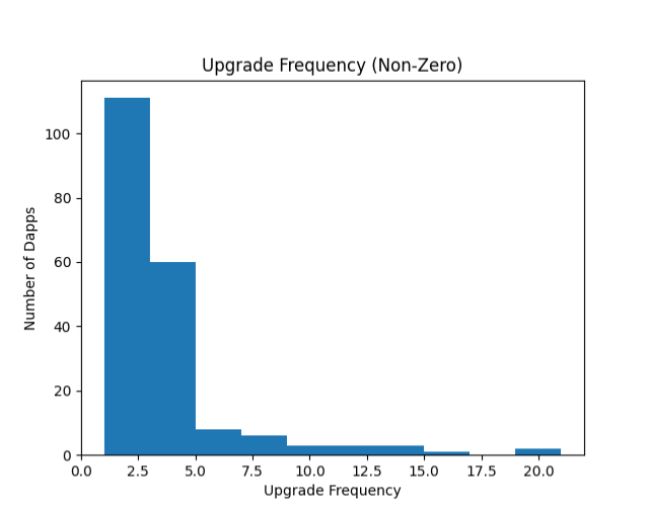
\includegraphics[width=0.45\columnwidth]{figures/UpgradeV26.png}\label{fig:upgradev26}}
      \qquad
      \subfloat[OpenZeppelin V3+]{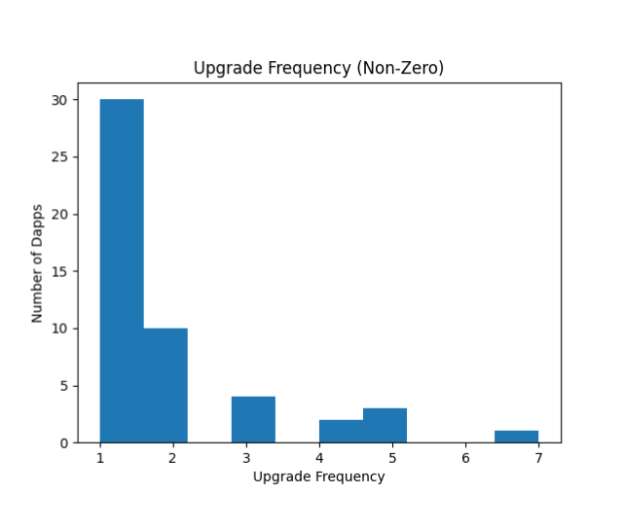
\includegraphics[width=0.45\columnwidth]{figures/upgradev3.png}\label{fig:upgradev3}}
  \caption{Number of Dapps (y-axis) over number of upgrades (x-axis) \label{fig:upgrade}}
\end{figure}
\begin{figure}[t]
  \centering
      \subfloat[OpenZeppelin V2.6]{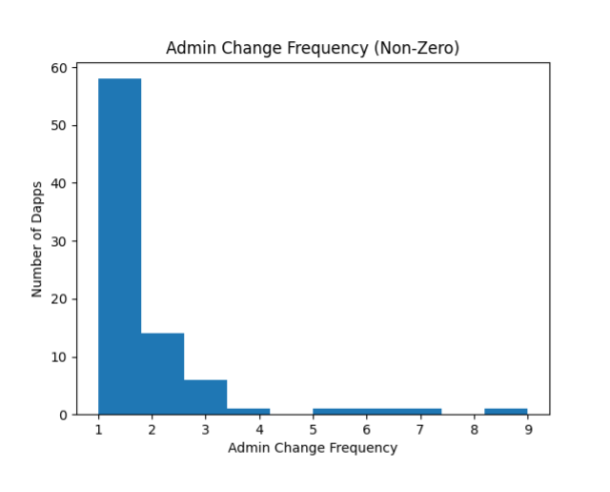
\includegraphics[width=0.45\columnwidth]{figures/Adminv26.png}\label{fig:adminv26}}
      \qquad
      \subfloat[OpenZeppelin V3+]{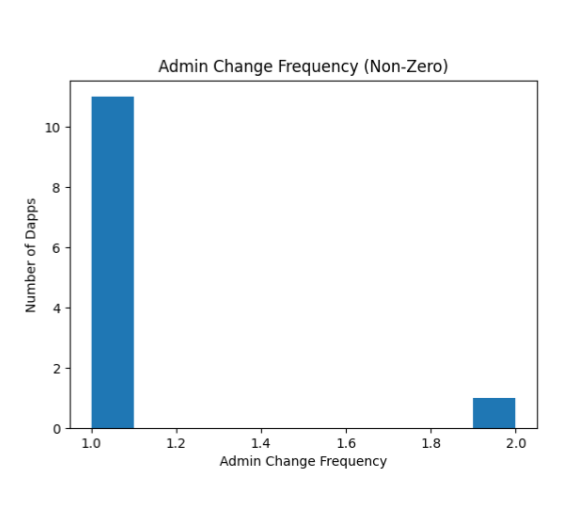
\includegraphics[width=0.45\columnwidth]{figures/Adminv3.png}\label{fig:adminv3}}
  \caption{Number of Dapps (y-axis) over number of Admin Changes (x-axis) \label{fig:admin}}
\end{figure}
The results for each version is:
\begin{itemize}
  \item For V2.6 (922 contracts):
  \begin{itemize}
    \item Upgrade Happens (see figure~\ref{fig:upgradev26}):
    \begin{itemize}
      \item 110 with One Upgrade, 60 with Two Upgrade, 2 with 20 upgrades, 5 with Five upgrade, 4 with 7 Upgrades, 3 with 10,12,15,16 Upgrades, 1 with 16 upgrades
    \end{itemize}
    \item Admin Change Happens (see figure~\ref{fig:upgradev3}):
    \begin{itemize}
      \item 57 with One Change, 14 with Two change, 4 with Three change, 1 with 4 changes, 1 Dapp with 5, 6,7,9 Changes
    \end{itemize}
  \end{itemize}
  \item For V3+ (309 contracts):
  \begin{itemize}
    \item Upgrade Happens (see figure~\ref{fig:adminv26}):
    \begin{itemize}
      \item 30 with One Upgrade, 10 with Two Upgrade, 4 with Three upgrade, 2 with 4 Upgrades, 3 with 5 Upgrades, 2 with 7 Upgrades
    \end{itemize}
    \item Admin Change Happens (see figure~\ref{fig:adminv3}):
    \begin{itemize}
      \item 11 with One Change, 1 with Two change
    \end{itemize}
  \end{itemize}
\end{itemize}


\textcolor{red}{Next section is the recent analysis which I used transaction based analysis to find proxy contracts.}



\subsection{Hybrid Analysis (Transaction and Bytecode based)}

In this part we focused on finding the \textit{Delegate-call} based upgradeable contracts. Before start explaining the process of finding upgradeable proxies, we describe why we focused on finding this pattern. 

\textit{Retail Change} methods is not possible to detect in large-scale. In \textit{Parameter change} method, one or multiple state variables can be changed inside the contract via a governance process. There is no distinction between a regular changeable state variable inside a contract and upgradeable one. The only way to detect these changes is reverse checking. In other words finding contracts that are govern the system and then find state variables that these governors can control. This way is possible for governance smart contract but not possible for Multi-Sig wallets and EOAs. 
\textit{Component Change} is very similar to parameter change method but here an address to another contract is changing. This method is not detectable in large scale as well because in this pattern the main contract calls another contract which does not have any specific patterns. This architecture is very regular in Ethereum blockchain so the only way to find them is reverse analysis that described above.

\textit{Wholesale change} approaches consist of \textit{Call-based}, \textit{Delegatecall-based} and \textit{Metamorphic} patterns. The Call-based pattern is an old fashion way of adding upgradeability to a system. This type is not used nowadays. On the other hand, \textit{Delegate-call}  pattern is widely used in ethereum contracts and this is the reason that we focused on this pattern. \textit{Metamorphic} pattern is very new and not well-tested yet. Also it has limitations such as the state of the contract should wiped out before upgrade each time because of need of self-destruction. Also there are some risks to this pattern. For instance there are discussions in Ethereum community about removing \textit{Selfdesctruct} opcode from EVM~\cite{selfDestruct}. 

In the above paragraph we claimed that the \textit{Call-based} pattern is not widely used these days. To prove this claim we perform an analysis on 93,000 verified smart contracts in smart contract sanctuary database~\cite{smart_contract_sanctuary}. As mentioned in previous sections \textit{Call-based} patterns consist of a logic contract and storage contract. The storage contract should define all storage variables needed for the system and must have getters and setters for these variables. Because the storage contract is not changeable in upgrade event the developers should be sure that all state variables that are needed are defined. One trick that give the developers ability to add new state variables after deployment is using \textit{Eternal Storage} pattern which described in previous version. This is the reason that why Eternal Storage is widely used in \textit{Call-based} patterns. In this analysis, we try to find contracts that uses eternal storage structure in their logic using Regular Expression analysis. \emph{470} contract are found that uses eternal storage patterns and then we filtered them to find contracts that uses eternal storage structure and only contains getter and setter functions and not other logics. After filtering the we come up with \emph{170} unique eternal storage contracts that are used as storage contract of upgradeable Dapps. The newest contract was deployed on 2018 which show that this pattern is not widely used these days.

In the further part of this section we focus on finding contracts that are using \textit{Delegatecall-based} patterns to add upgradeability feature.



In the further sections we describe the \textit{methodology} of our work, the \textit{implementation} of the methodology and the \textit{results}.  

\subsubsection{Methodology}
As mentioned in classification section, the \textit{DelegateCall-based} upgradeability approach consists of a storage contract (a.k.a proxy contract) and a logic contract (a.k.a implementation contract). 

Proxy contract is a simple type of smart contract in which there is a fallback function. Fallback function is a function inside a smart contract that do not have a function name. It means if a user sends a transaction to the contract including a call to a function that does not exists on the contract, it will passed into the fall back function and the logic inside the fall back function will be executed. So if a user calls a contract with a function signature that does not exist on that contract, it is equal to calling the fallback function.

Inside the fall back function of the proxy contracts, there is a delegate call to the address of \textit{implementation contract} and pass the input data of the transaction to the implementation contract without altering it. In the rest of the paper, we we call implementation address inside the proxy, \emph{Target address}.

All proxy contracts have the above structure. But \textit{Upgradeable proxy contracts} should have another extra condition as well. The agent that responsible of changes in the smart contract contract (a.k.a \emph{admin}) must have the ability to change target address inside the proxy. If a proxy does not have this condition, it means that the contract is just forwarding the calls into a fixed implementation contract for the rest of its life and so, this proxy is not upgradeable. There are bunch of patterns that follows this structure (e.g. Minimal Proxies, Delegate call forwarders, etc.) which we call them \textit{Forwarders} in the rest of the paper. So, for upgradeable proxies the target address should be changeable.

Collecting transactions and information regarding these transaction, we filter transactions to the proxy contracts by checking if these transactions pass a fallback function which delegate calls the message data into another contract without any changes.

As discussed above, these proxies can be forwarders or upgradeable proxies. To find upgradeable proxies we should filter them by checking whether the target address is changeable for the proxy contract or not.

We first check if the target address comes from an external call to another contract. If yes we should just check that callee contract that if the target address inside it is changeable. If yes the proxy contract is \textit{Beacon Proxy} contract. In this case our proxy contract grabs the target address from another contract (a.k.a Beacon contract) each time and because this address is changeable inside the beacon contract, the admin can just change this address from the beacon contract and upgrade the system whenever they want.

If the address does not come from an external call, then we check if the there is any function or way to change the target address inside the proxy itself. If yes then our proxy is an upgradeable proxy because the admin can just change the target address through that function inside the proxy and upgrade the system.

If there is no way to change the target address inside the proxy, then we pass it to another filter. There is another way of implementing upgradeable contracts named \textit{Universal Upgradeable Proxy Standard (UUPS)} that discussed in previous parts. In this method, the target address is changeable using the implementation contract. So to filter and find them, we check the implementation contract to find out if there is any function inside the implementation contract that the admin can change the target address using that function. If yes then our proxy is UUPS proxy other wise the proxy is not upgradeable.

The whole process is depicted on figure~\ref{flowchart}.

\begin{figure}[t]
  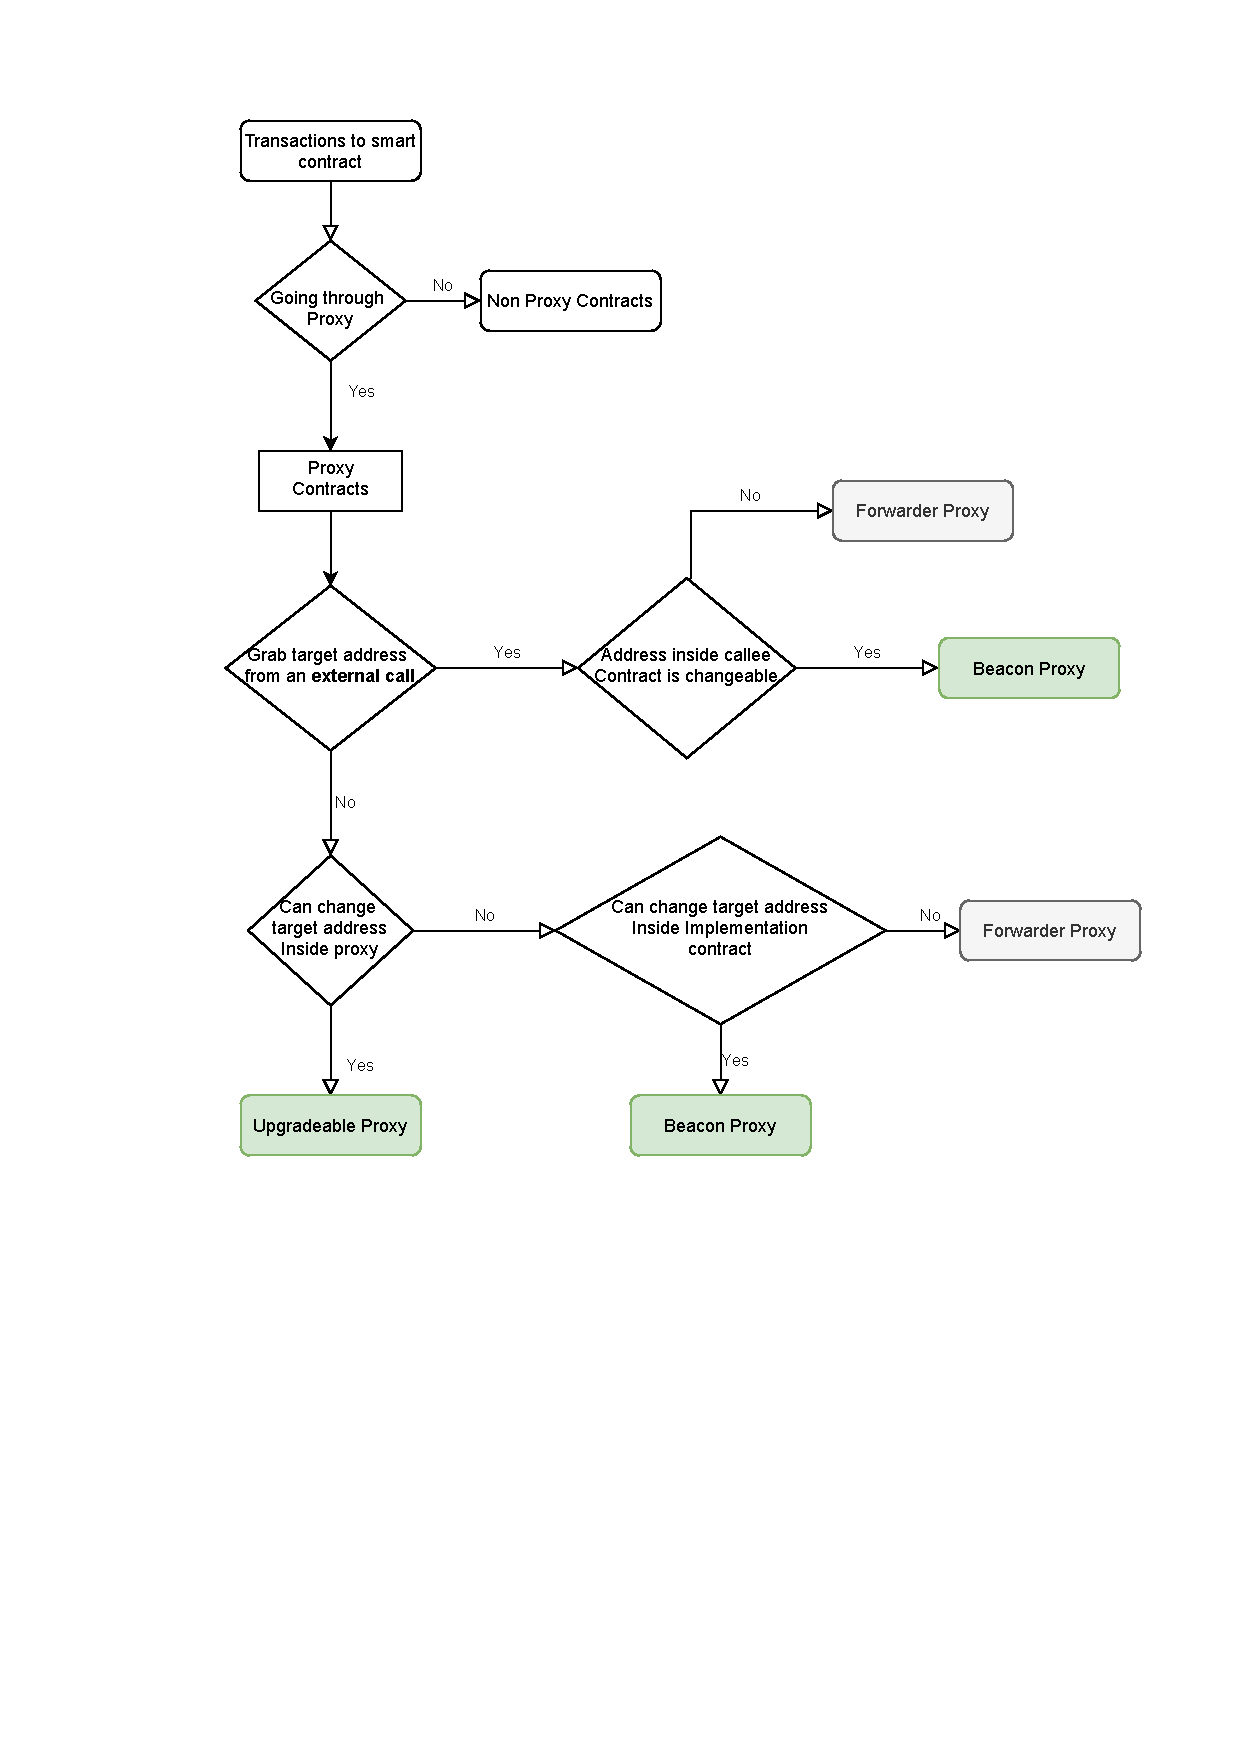
\includegraphics[width=0.8\textwidth]{Methodology.pdf}\label{flowchart}
  \caption{Flowchart of the Process}
\end{figure}


\subsubsection{Implementation}
In this section we describe the processes of finding upgradeable proxy contracts explained in the previous section in detail of implementation and execution. 
Each block of Ethereum blockchain is consist of transactions that processed in that exact block. To get all transaction details we need to replay the transaction and collect the data of execution. Ethereum full archival node has a method, \textit{trace\_transaction},  that gives the \textit{Parity VM transaction traces} inside an specific block. Each transaction trace is composed of actions that each of them consists of an opcode relevant to the code of smart contract and the transaction that is sent to the blockchain and manipulate the state, memory or stack of the Ethereum blockchain. 

Having the transaction traces for each block, we will search to find actions that consists of \textit{callType} . If the trace consists of callType element it means that a \textit{Call},\textit{Static Call} or \textit{Delegatecall} happened in that action. we picked actions that have \textit{callType} and this call type is \textit{delegate call}. Also each action has an \textit{input} element for messages that have a call data. If the input element of the selected actions are equal to the input element of their previous action it will be interpreted as the transaction goes through a fallback function that delegate calls it to another contract. Because the input or call data is not changed, in the delegate call it means that there is no function with the function selector specified by the input on the smart contract and so the transaction went into a fallback function. Also because there is a delegate call into another contract with the same input it means that inside that fallback function there is a delegatecall that passes the whole message data to the target address contract.So, these contracts meet our first condition that described above and we mark them as \textit{Proxy Contracts}and collect \textit{From address},\textit{To address} and the \textit{transaction hash} of these picked actions and pick the unique from addresses of this data. From address is the address of sender of transaction, to address is the address which the proxy sends the transaction into and transaction hash is the transaction identifier that is used in Ethereum blockchain. 

As discussed before, these selected contracts are proxy contracts and not necessarily upgradeable proxy contracts. So, we need to filter the forwarders from proxy contracts to find upgradeable proxy contracts. As mentioned in methodology section, the upgradeable proxy contracts must have a condition; the admin of the contract should be able to change the target address. In other words, we should check if the target address inside the proxy contract is changeable or not.

Five regular ways for the situation that the target address is fixed and not changeable on the contract:
\begin{enumerate}
  \item The target address is hardcoded in the contract without assignment to any variables
  \item The target address is saved in a constant or immutable variable type 
  \item The deployer adds the target address via a constructor function
  \item The target address is defined in a storage variable, but there is no function or a way to change this address after contract deployment
  \item The proxy contract grabs the target address each time by calling another contract and there is no way on the callee contract to change this address
\end{enumerate} 

In the first three situations, the target address amount will be appeared on the bytecode of the smart contract. So, we can get the bytecode of each proxy contract that are collected from previous part using the \textit{eth\_getCode} method of a Ethereum archival node. Then we need to check if the target address is appeared on the bytecode or not. To have the target addresses we just need to collect The \textit{To addresses} that we collected on the previous part which are supposed to be the implementation addresses because the proxy contract delegate calls into these addresses. So we easily checked if the \textit{To addresses} are appeared on the bytecode of the \textit{From addresses} (which is the proxy contract's bytecode). If yes, these proxies are not upgradeable proxies and they are forwarder contracts.

For the situation 4, we need other processes to check whether the implementation address is changeable or not. We need to design a filter to tell us is there a way to change the target address or not. We will describe the filter in the later part of the paper, but for now let's assume that we have a filter module named \textit{Assignment Checker} that checks and tells us that whether there is a function inside the proxy contract that can change the target address by calling a function. If yes mark the contract as an upgradeable proxy contract. So, now we have output addresses that their contract has fall back functions that delegate calls the whole data into another implementation contract and their target address is changeable on the proxy contract. So, we have a dataset of upgradeable proxy contracts.

For the situation 5, we check the proxy contracts to find if the target address inside the proxy contract is coming from an external call to another contract. If yes the we check the callee smart contract (a.k.a Beacon contract) that if the target address is changeable inside that contract or not. If it is changeable we mark the proxy as \textit{Beacon Proxy} otherwise it is a \textit{Forwarder}. 

But this is not the end of story. There is another proposed upgradeable proxy contract pattern, named Universal Upgradeable Proxy Standard (UUPS) also known as EIP-1822 that described in the previous sessions. In this type of proxy contracts, the amount of target address is changeable using the implementation smart contract. As mentioned above the code of the implementation contract is executed in the context of the proxy contract and so it will change the storage state of the proxy contract. If we have a function in the implementation contract that gives us the ability to change the storage slot of the target address inside the proxy contract's storage, we can upgrade the system by calling that function of implementation contract. We couldn't catch this type of upgradeable contracts by the previous processes because we just checked if there is a function inside the proxy contract that can change the target address.

We can tackle this problem by first finding the storage slot inside proxy contract in which the implementation address is recorded. Then check if the admin of the implementation contract can change the variable defined on that specific storage slot using a function inside the implementation contract. So first we should find the storage slot of the proxy contract in which the target address is saved. There are two EIPs out there that makes it easy to find these storage slots that should be used  to save target address for upgradeable proxies; EIP-1967 \footnote{0x360894a13ba1a3210667c828492db98dca3e2076cc3735a920a3ca505d382bbc} and EIP-1822 \footnote{0xc5f16f0fcc639fa48a6947836d9850f504798523bf8c9a3a87d5876cf622bcf7}.suggested randomly selected storage addresses for implementation addresses to mitigate the overwriting on these slots. The general way to do this is not using these proposed slots from these EIPs for this process. The general way is to find the storage slot from the proxy contract and then check if admin can change this specific storage slot inside the implementation contract. But this way is not doable in large scale because in \textit{Assignment checker} module we need to decompile the bytecode which is time consuming for contracts that have a large bytecodes. Implementation contracts are usually large pieces of codes. So, it is not possible to do this process in a large-scale for all proxy contracts that are found from the previous parts. This is the reason that we limit our filter to specific storage slots proposed in EIP 1967 and EIP 1822.

So for this part we use the remained proxy contract addresses from the previous part. First we select the contracts that their target address is saved on the specific storage slots mentioned above and if yes check the implementation contract to find variable regarding that storage slot. Afterwards check if the variable is changeable via implementation contract. As mentioned before, the \textit{To addresses} are the implementation contracts. We first find the variable in the implementation contract that is saved in the mentioned slots. Then pass it to our filter \textit{Assignment Checker} to check if the admin of the contract is able to change it or not. If it is changeable, it means that the admin can upgrade the system using a function on the implementation contract, and so the proxy is an UUPS contract. 

The whole process is depicted on figure~\ref{fig:finderModule}.

\begin{figure}[t]
  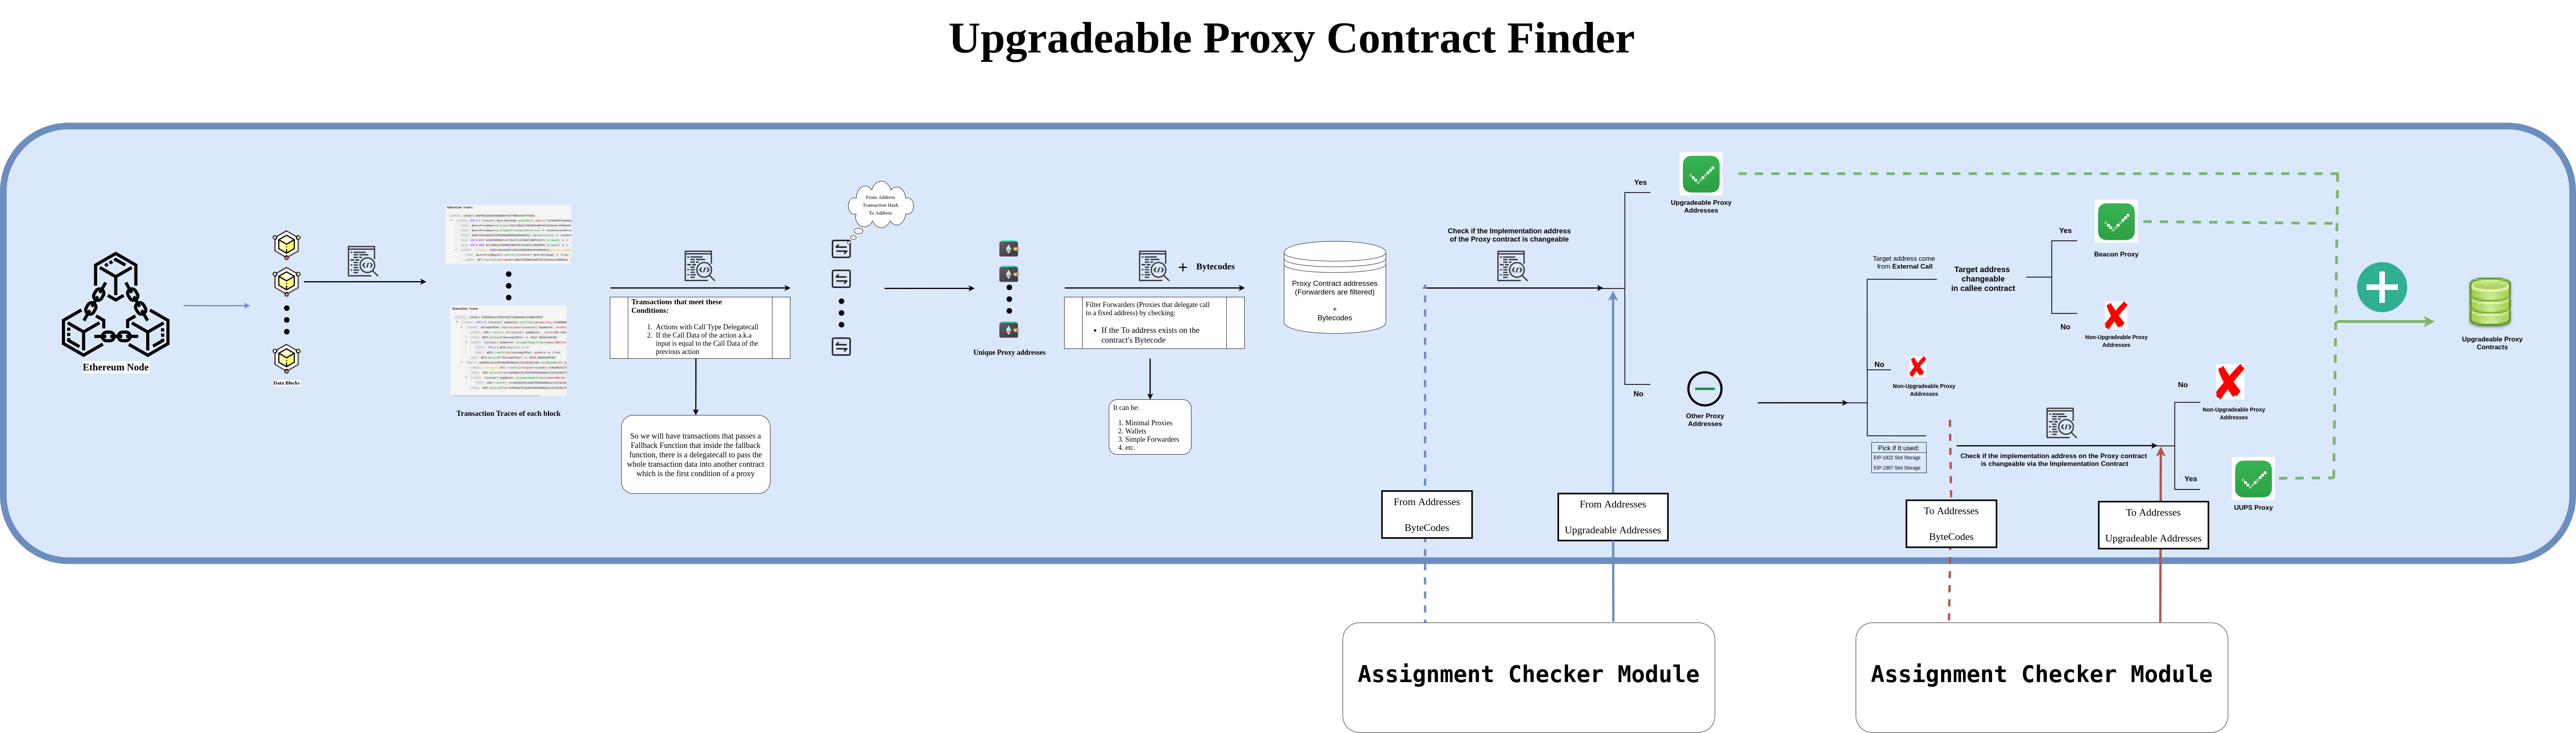
\includegraphics[width=0.8\textwidth]{figures/Upgradeability_finder1.png}\label{fig:finderModule}
  \caption{Upgradeability Proxy Contract Finder}
\end{figure}

\subsubsection{Assignment Checker Module}

As mentioned in the previous part, we need a module to check if the admin can change target address on the proxy contract, implementation contract or beacon contract. For this purpose we need a module that gets \textit{{Bytecode}} of the proxy/implementation address as input and find the variable name and storage slot of the variable that the target address is saved into it and then check to find out is there any function inside the contract that gives the admin the ability to change the target address.

We use bytecode decompiler named \textit{Panoramix decompiler} to decompile the bytecodes into well-formated python language codes. The decompiled code gives us all storage variables and their storage slots in a function named \textbf{Storage}. On the other hand, the decompiled code will tell us if a function is \textit{Payable} or not. Among these Payable functions the one that does not have name or its name is fallback is the \textit{fallback} function of the contract. So we will try to find the line that \textit{Delegate Call} happened on it and collet these lines. Now that we have storage variable names and storage slots of these variables and also the line of code inside fallback that have the delegatecall, we will check to find the target address variables. We are doing that by checking if one of the storage variables is used inside the line of code that contains delegation. 
% or if there is a hash a text is inside the line of the code (if there is 'sha3' inside the line). 

There is two other steps here. First if there is a variable name in the storage function of decompiled code that has the same slot with implementation variables we captured from previous part we will add those variables to target address variables. Also if we find another variable that being assigned to captured target address variables, we will add them to the implementation addresses as well.

Now that we have a list for target variables, we will search through the code to find if any assignment happened to one of them. If yes we will pick the variables that is assigned to target variable and then check if this picked variable is the input of the function in which the assignment occurred. If yes it means that there is a function that the admin can change target address using this function.

To summarize what we did, we find all possible variables in the code that can change the target address inside the proxy/implementation contract and check if there is any function inside them that can alter the implementation address.

The whole process is depicted on figure~\ref{assignmentFinder}.

\begin{figure}[t]
  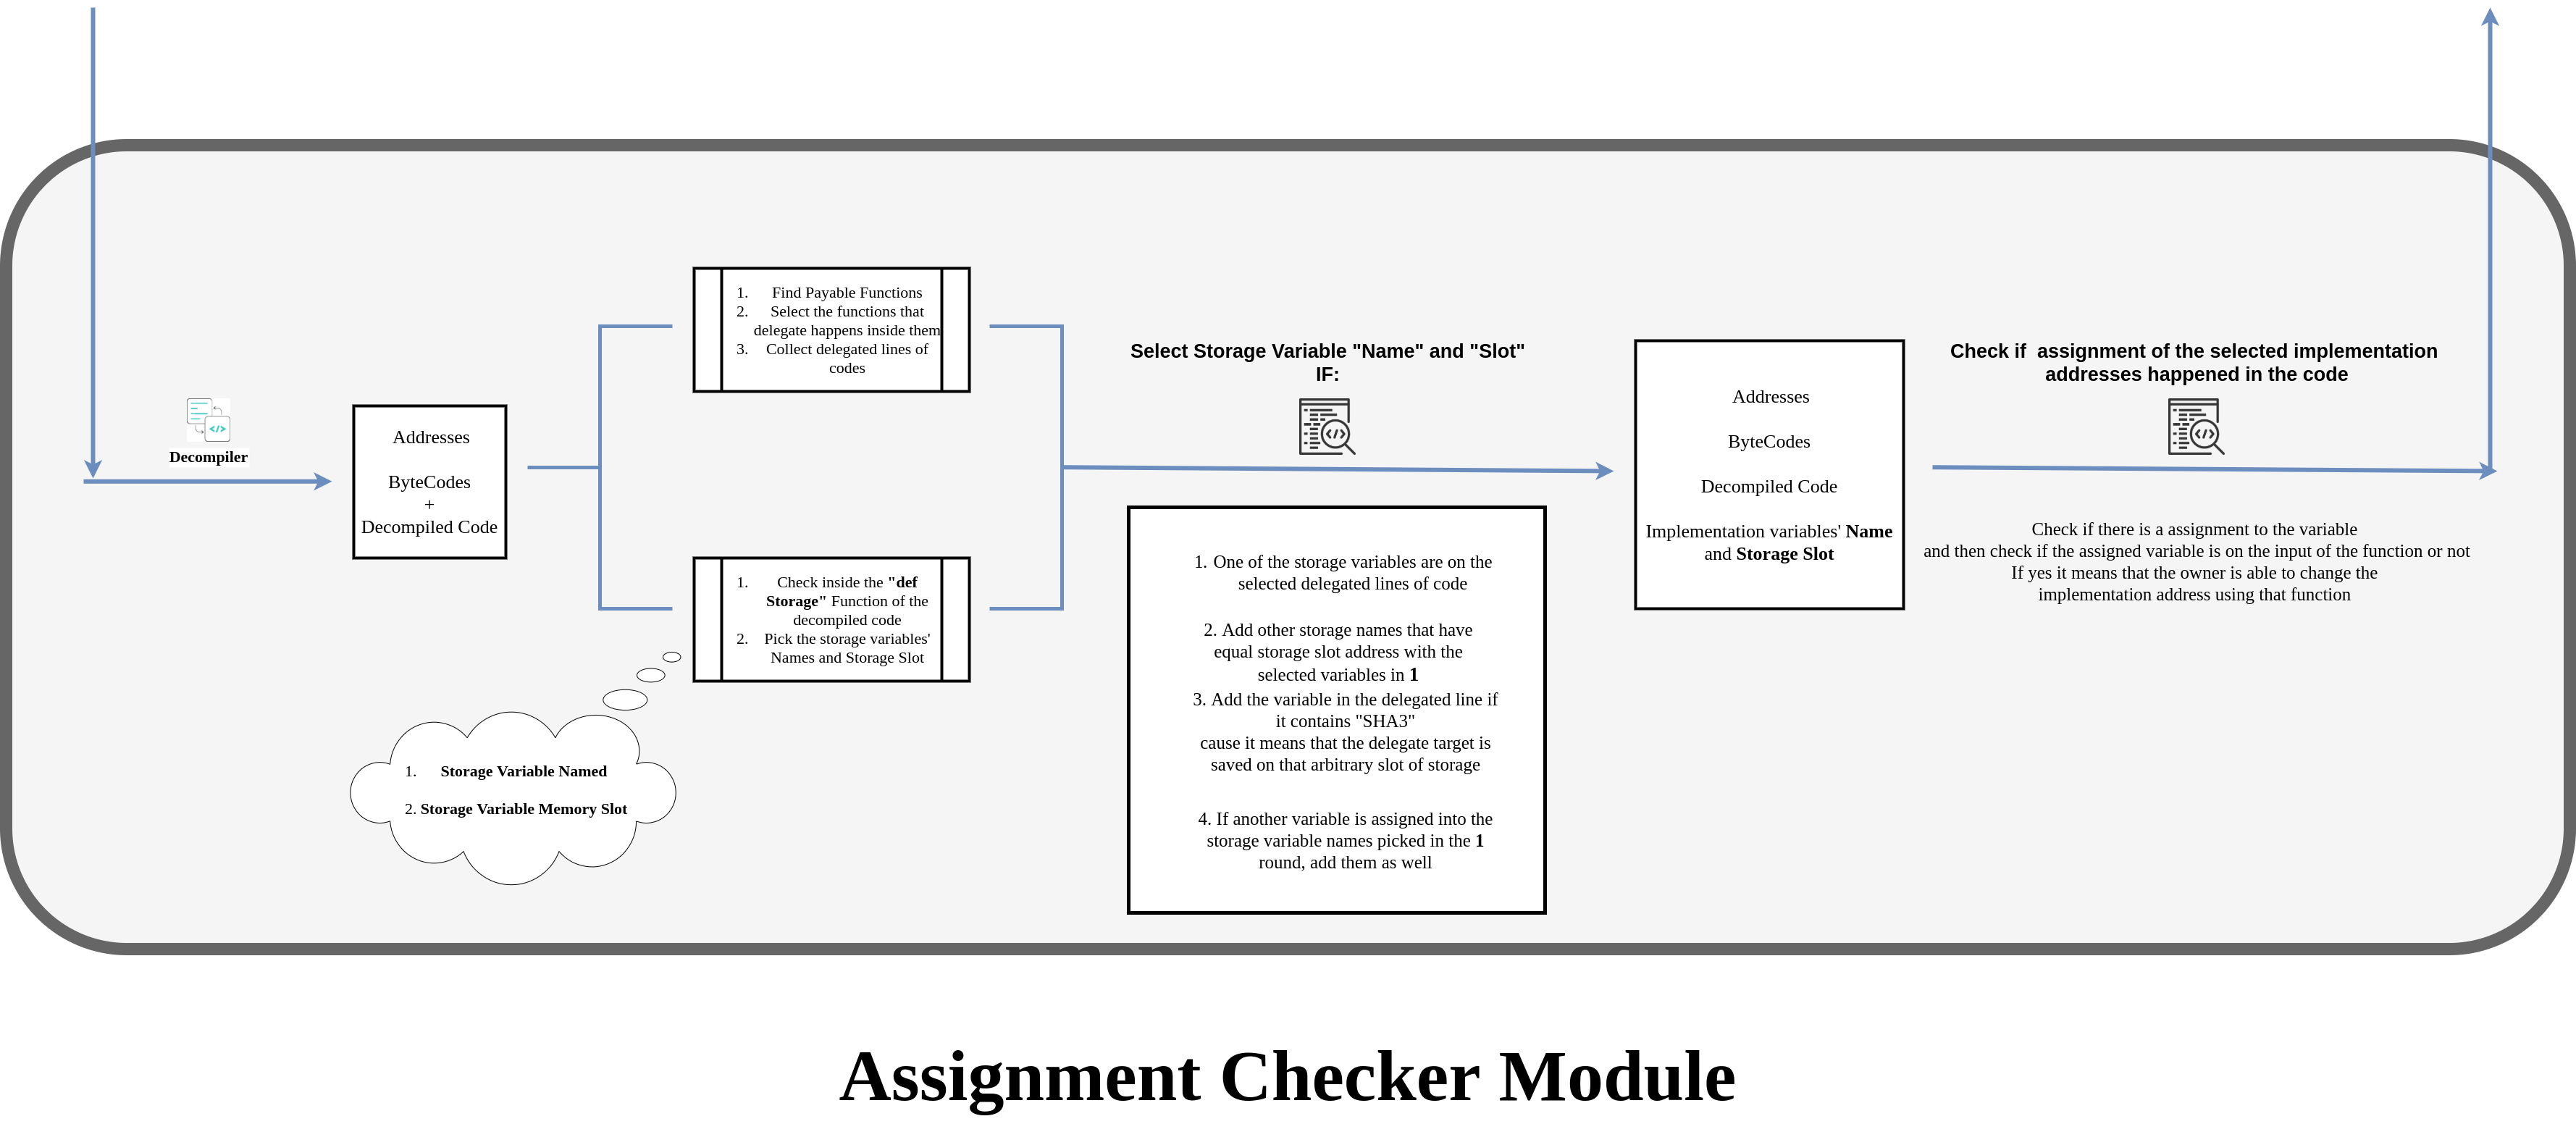
\includegraphics[width=0.8\textwidth]{figures/Assignment_finder.png}\label{assignmentFinder}
  \caption{Assignment CheckerModule}
\end{figure}



\subsubsection{Results}
Having access to an Ethereum full archival node we have collected transaction traces of transactions included in 2,064,595 blocks of Ethereum blockchain, starting from block number \textit{\#10800000} to \textit{\#12864595}. It covers transactions on the Ethereum blockchain from \textit{Sep-05-2020} to \textit{Jul-20-2021}. 

Having transaction traces and the actions of each transaction, we have collected \textit{From} address (address of sender of the transaction), \textit{To} address (destination address of the transaction) and \textit{Transaction Hash} of actions which has \textit{delegateCall} as their \textit{Call Type} that their input is the same as their previous action.

To have the proxy contract, we find the unique From addresses from all collected transactions which gives us \textit{1,427,215} unique proxy contracts. But bunch of these proxies are using a shared implementation contracts. So after filtering proxies with the same implementation contracts we come up with \textit{13,088} contracts.

Afterwards we filter \textit{Forwarder Contracts} from our data set by checking if the To address appears on the contract's bytecode and then pick the upgradeable proxy contracts by checking if implementation addresses is changeable inside their code. Totally we find \textit{7,470} regular upgradeable proxy contracts. 

On the other hand, we checked the remained proxy contracts to find out if their implementation address is based on EIP-1822 or EIP-1967 proposed storage slots. On these selected contracts we picked their implementation address contract and check if the implementation address is able to change the implementation address on the proxy contract, if yes we mark the address as upgradeable proxy contract. The outcome of this last filter is \textit{403} upgradeable proxy contracts that uses Universal Upgradeable Proxy Pattern. Also our code result shows \textit{352} unique beacon proxy contracts as a result as well.

At the end we have \textit{8,225} upgradeable proxy contracts. We randomly sampled 150 contracts from these contracts and manually check them and all of them were upgradeable proxy contract. On the other hand, we sampled 150 contracts from the contracts that marked as non-upgradeable contracts and check them manually. between these 150 contract just two of them was upgradeable and it was a false-negative. The reason that our model did not catch this contract was failure happened on the decompiler to decompile the implementation contract code and so assignment checker detector could not catch them. 

\subsubsection{Attacking Universal Upgradeable Proxy Standard (UUPS) contracts}
In the previous sections \ref{sysComplexity} (in Delegate-call section) we discussed that the implementation function should not contain \textit{constructor} function and instead of that there should be regular function namely \textit{Initialize} function that can be called just once and has the same functionality as constructor function. So the contract creator must call initialize function through proxy contract quickly after deploying the proxy contract. The Initialize function does not have any access control because it is considered to be called once and this function is responsible to define the owner so before calling this function we don't have the owner's address to check it for access control of the function. This is the main reason that there should be a check to be sure that this function can just be called once and not more. Regularly, the deployer (the dev team) will define and initialize the owner of the contract (address which have the control of upgrading the system) via initialize function. So if the initialize function can be called more than once, or the deployer do not initialize the contract, then any external address can call initialize function and change the owner of the contract and take control of the contract. But this is not the case and less likely to happens because this is the first row of checklist of this type of upgradeability pattern.

There is another important issue that should take care of. We talked about calling the initialize function through proxy contract. But what about calling this function directly from the implementation contract itself? If the deployer do not call the initialize function directly from implementation contract to initialize it once (and to lock it), then any malicious address can call this function from implementation contract and change the owner inside the implementation contract and take control of the implementation contract. But one can ask what is the issue if another person takes control of the implementation contract. The answer depends on the functions inside the implementation contract and what executions can be done by the owner. If the functions inside implementation contract just change the state, then the attacker cannot attack the system because he/she just can change the state inside the implementation contract and our Dapp relies on the data that are saved inside proxy and not the data inside the implementation contract.

But it is not end of story, if the owner of the implementation contract has ability to self-destruct the contract, then the attacker can use initialize function inside the implementation contract to take control of the contract, and self-destruct it. This type of attack is a Denial of Service attack because transaction which are sent to proxy will be delegate called into a self-destructed contract and cannot peruse the desired logic. There is another way for attacker to self-destruct the implementation contract even if the contract itself does not have a self-destruct inside it. In case that the implementation contract has a function in which it delegate calls to another contract, and the target address of this delegate call can be changed by owner, then the attacker can take control of the owner's address using initialize function and then change the target address in the implementation contract and then call the function that delegate calls to the malicious address. The attacker can implement self-destruction inside the malicious contract and so, when the implementation contract delegate calls the malicious contract which executes self-destruct the implementation itself will be self-destructed like the previous scenario. 

If the Dapp has an upgrade function inside its proxy contract, then the owner of proxy can just upgrade the proxy into a new version of implementation contract, This attack is explained in December 2020 by Trail of Bits team when they audit the code of Aave, a lending project~\cite{aaveBreak}.

There is another scenario which is more detrimental than the explained scenario. As mentioned in the previous sections in UUPS upgradeable contracts, the upgrade function resides in the implementation contract and so there is no way to upgrade the system by proxy itself. So if an attacker can take control of the implementation contract by calling initialize function directly from implementation contract, and then self-destruct it, there is no way to upgrade the system and consequently the proxy will be locked forever. All UUPS contracts that used Openzepplin UUPS library and their implementation contact do not get initialized is susceptible to this attack because there is a function in implementation contract of this library \textit{upgradeToAndCall} in which the owner can change a target address and then delegate call into the newly changed target address. This attack vector was found in September 2021 and announced by OpenZepplin team~\cite{securityAdvise}\cite{uupsAttacks}. There is an easy way to mitigate this attack just by calling initialize function directly from implementation contract. 

We try to check all UUPS contracts that we have to find if any of them can be exploited in this way. We check all of them manually and the method of checking them is described bellow:

\begin{enumerate}
  \item Find initialize function inside the implementation contract
  \item check if anybody can call this initialize function directly from implementation contract and change the owner of the contract
  \begin{itemize}
    \item Filter ones that are already initialized and so locked (which means that the initialize function is not callable)
    \item Filter those ones that have a modifier that blocks direct calls from the implementation contract (there is modifier that lets just transactions that come from proxy contract and blocks direct calls from implementation)
  \end{itemize}
  \item Check if there is a way inside the implementation to self-destruct 
  \item Check if there is a function inside the implementation contract in which there is a delegate call to another target address
  \item Check if the target address is changeable 
\end{enumerate}

Checking the list above we find 15 contracts in our data set which were exploitable till September 9, 2021 and openzeppelin team patched them by initializing the contract. It means that an attacker could deploy a new malicious contract which executes self-destruct on any calls to it. Then take control of the implementation contract by calling initialize function of them. Afterwards, the attacker should find the function inside the implementation contract that have a delegate call inside it and find the target address. There should be a function inside implementation contract to change the address to the malicious contract that the attacker deployed recently and just after that the attacker call the function to execute a delegate call into the malicious contract and then self-destruct the implementation contract.

We find 61 UUPS contracts that are not initialized and anybody can take control of these implementation contracts but because these contracts do not use delegate call or self-destruct, they are not exploitable by this type of attack.

\subsubsection{Rug Pools (Exit Scams)}


% Level of intervention of each Dapp (pauseable etc.)
% History of upgrades --> How many times a Dapp upgraded before (using events etc...)

% \section{Concluding Remarks}


% \subsection{Registry pattern}
% Registry contracts are probably the simplest approach to upgradeability. Registry pattern consist of two main contracts: registry and logic contract. Registry contract holds the addresses of logic contracts and whenever it receives a transaction it will pass it to the related logic contract. 
% If the development team decide to upgrade the smart contract, they can deploy another smart contract and then just change the pointer of the registry smart contact to the new smart contract.

% The main disadvantage of this approach is that in upgrading event, there should be a manual or automated migration plan to transfer data from the old contract into the new upgrade smart contract.
% Another drawback of this pattern is that it also introduces additional complexity for external clients who would also need to call into the registry before interacting with the system


%Idea: see how frequent each project uses its upgradeability feature to upgrade the contract and why?

%In proxy storage layout you should take care that: 
% 1. never remove variable
% 2. never change var type
% 3. never change inheritance order


%Implementation of Eternal storage in call based upgrades: https://medium.com/cardstack/upgradable-contracts-in-solidity-d5af87f0f913
% Good classificaton: https://medium.com/1milliondevs/solidity-storage-layout-for-proxy-contracts-and-diamonds-c4f009b6903
% New storage type *Dimond Storage*: https://medium.com/1milliondevs/new-storage-layout-for-proxy-contracts-and-diamonds-98d01d0eadb
%https://medium.com/1milliondevs/new-storage-layout-for-proxy-contracts-and-diamonds-98d01d0eadb
% Upgradability checklist: https://blog.trailofbits.com/2020/06/12/upgradeable-contracts-made-safer-with-crytic/



%ToDo: Write about OpenZeppelin upgrade bug : https://blog.trailofbits.com/2018/09/05/contract-upgrade-anti-patterns/
%ToDo: Gas cost comparison between different implementation (using different number and types of the storage variables)


\section{discussion}
%\subsection{Off chain upgrades (UNiswap Arbitrum)}: On-chain voting for an off-chain process. Other types of upgrade. Like front end changes etc.

% !TEX root = ../main.tex

\begin{table}[t!]
    \centering
    
        \begin{tabular}{lllllllllllllll}
    
    &
    \headrow{Can replace entire logic} &
    
    \headrow{can replace pre-specified part of logic} & 


    \headrow{Can replace entire state} &
    
    \headrow{can change pre-specified state variables} &
    
    \headrow{No need to deploy a new contract} &

    \headrow{No need to migrate state from old contract} &

    \headrow{No need to separate State and Logic} &

    \headrow{Function Selector Clashes Risk} &

    \headrow{Storage Clashes Risk} & 

    \headrow{No indirection} & 


    \headrow{User endpoint address not changed} &
    

    \headrow{Downtime in upgrade events} &

    \headrow{No need to change code to add the upgrade pattern} &

    \headrow{Need to change a state variable} 
    
    
    \\
    
    \hline
 
    
        \multicolumn{1}{c|}{Parameter change}	& \multicolumn{1}{c|}{}  & \multicolumn{1}{c|}{} &  \multicolumn{1}{c|}{} & \multicolumn{1}{c|}{\checkmark} & \multicolumn{1}{c|}{\checkmark} & \multicolumn{1}{c|}{\checkmark} &  \multicolumn{1}{c|}{\checkmark} &  \multicolumn{1}{c|}{} & \multicolumn{1}{c|}{} & \multicolumn{1}{c|}{\checkmark} & \multicolumn{1}{c|}{\checkmark} & \multicolumn{1}{c|}{} &\multicolumn{1}{c|}{\checkmark} & \multicolumn{1}{c}{\checkmark}\\
    
        \hline
  
        \multicolumn{1}{c|}{Component Change}	& \multicolumn{1}{c|}{}  & \multicolumn{1}{c|}{\checkmark} &  \multicolumn{1}{c|}{} & \multicolumn{1}{c|}{} & \multicolumn{1}{c|}{} & \multicolumn{1}{c|}{\checkmark} &  \multicolumn{1}{c|}{\checkmark} &  \multicolumn{1}{c|}{} &  \multicolumn{1}{c|}{} &  \multicolumn{1}{c|}{\XBox} & \multicolumn{1}{c|}{\checkmark} & \multicolumn{1}{c|}{} & \multicolumn{1}{c|}{\XBox} &  \multicolumn{1}{c}{\checkmark}\\
        

        \hline

        \makecell{Migration}	& \multicolumn{1}{|c|}{\checkmark}  & \multicolumn{1}{c|}{} &  \multicolumn{1}{c|}{\checkmark} & \multicolumn{1}{c|}{} & \multicolumn{1}{c|}{} & \multicolumn{1}{c|}{} &  \multicolumn{1}{c|}{\checkmark} &  \multicolumn{1}{c|}{} &  \multicolumn{1}{c|}{} &  \multicolumn{1}{c|}{\checkmark} & \multicolumn{1}{c|}{} & \multicolumn{1}{c|}{} & \multicolumn{1}{c|}{\checkmark} &  \multicolumn{1}{c}{}\\
    
         \hline


        \makecell{Call-based}	& \multicolumn{1}{|c|}{\checkmark}  & \multicolumn{1}{c|}{} &  \multicolumn{1}{c|}{} & \multicolumn{1}{c|}{} & \multicolumn{1}{c|}{} & \multicolumn{1}{c|}{\checkmark} &  \multicolumn{1}{c|}{} &  \multicolumn{1}{c|}{} &  \multicolumn{1}{c|}{} &  \multicolumn{1}{c|}{} & \multicolumn{1}{c|}{} & \multicolumn{1}{c|}{} & \multicolumn{1}{c|}{} & \multicolumn{1}{c}{\checkmark}\\
    
        \hline


        \makecell{DelegateCall-based}	& \multicolumn{1}{|c|}{\checkmark}  & \multicolumn{1}{c|}{} &  \multicolumn{1}{c|}{} & \multicolumn{1}{c|}{} & \multicolumn{1}{c|}{} & \multicolumn{1}{c|}{\checkmark} &  \multicolumn{1}{c|}{} &  \multicolumn{1}{c|}{\checkmark} & \multicolumn{1}{c|}{\checkmark}&  \multicolumn{1}{c|}{} & \multicolumn{1}{c|}{\checkmark} & \multicolumn{1}{c|}{} & \multicolumn{1}{c|}{\XBox} & \multicolumn{1}{c}{\checkmark}\\

        \hline

        \makecell{Diamonds}	& \multicolumn{1}{|c|}{\checkmark}  & \multicolumn{1}{c|}{} &  \multicolumn{1}{c|}{} & \multicolumn{1}{c|}{} & \multicolumn{1}{c|}{} & \multicolumn{1}{c|}{\checkmark} &  \multicolumn{1}{c|}{} &  \multicolumn{1}{c|}{\checkmark} & \multicolumn{1}{c|}{\checkmark\checkmark}&  \multicolumn{1}{c|}{} & \multicolumn{1}{c|}{\checkmark} & \multicolumn{1}{c|}{} & \multicolumn{1}{c|}{\XBox} & \multicolumn{1}{c}{\checkmark}\\
        
        
         \hline

        \makecell{Metamorphic}	& \multicolumn{1}{|c|}{\checkmark}  & \multicolumn{1}{c|}{} &  \multicolumn{1}{c|}{\checkmark} & \multicolumn{1}{c|}{} & \multicolumn{1}{c|}{} & \multicolumn{1}{c|}{} &  \multicolumn{1}{c|}{\checkmark} &  \multicolumn{1}{c|}{} & \multicolumn{1}{c|}{}&  \multicolumn{1}{c|}{\checkmark} & \multicolumn{1}{c|}{\checkmark} & \multicolumn{1}{c|}{\checkmark} & \multicolumn{1}{c|}{\checkmark} &  \multicolumn{1}{c}{}\\
        
        
         \hline
        
        
        \end{tabular}
        \captionsetup[tabular]{singlelinecheck=off}
        \caption{Evaluation}
       
    
    \end{table}
    \footnotetext[1]{Design of system in which a parameter can change the logic is hard}